\documentclass[times, twoside]{zHenriquesLab-StyleBioRxiv}

\usepackage{newfloat}
\DeclareFloatingEnvironment[name={Supplementary Figure}]{suppfigure}
\DeclareFloatingEnvironment[name={Supplementary Table}]{supptable}
\usepackage{multirow}
\usepackage{makecell}
\usepackage{upgreek}

\newcommand{\dreca}{$\Delta$\textit{recA}} % ΔrecA
\newcommand{\teneighty}{RecB$_{1080}$} % RecB1080
\newcommand{\geneteneighty}{\textit{recB$_{1080}$}} % recB1080
\newcommand{\od}{OD$_{600}$} % OD600
\newcommand{\umsq}{$\upmu$m$^2$} % µm2
\newcommand{\ums}{$\upmu$m$^2$.s$^{-1}$} % µm2.s-1
\newcommand{\ncells}[1]{N$_{\text{cells}}$ = #1} % N_cells = {}
\newcommand{\nspots}[1]{N$_{\text{spots}}$ = #1} % N_spots = {}
\newcommand{\nnucl}[1]{N$_{\text{nucleoids}}$ = #1} % N_nucleoids = {}

% Surname of the lead author for the running footer
\leadauthor{Thédié} 

\begin{document}

\title{RecBCD dissociation from DNA \emph{in-vivo} is independent from external factors}
\shorttitle{}

\author[1]{Daniel Thédié}
\author[2]{Alessia Lepore}
\author[1]{Lorna McLaren}
\author[1]{Meriem El Karoui}


\affil[1]{Institute of Cell Biology, University of Edinburgh, Edinburgh, UK}
\affil[2]{Ecole Polytechnique, Paris-Saclay, France}

\maketitle

\begin{abstract}
Abstract text will come here.
\end{abstract}

\begin{keywords}
DNA repair | RecBCD | Imaging | \emph{in-vivo}
\end{keywords}

\begin{corrauthor}
meriem.elkaroui\at ed.ac.uk
\end{corrauthor}


\section*{Introduction}
% RecBCD biochemistry
Repairing DNA damage and ensuring integrity of the genome is essential to all living organisms. Among the different types of damage, DNA double-strand breaks (DSBs) pose a serious threat to bacterial cells: when left unrepaired, they can lead to cell death, genome rearrangements or mutagenesis \cite{Wyman2006}. In \ecoli, DSBs are repaired through the RecBCD pathway. RecBCD is a heterotrimeric protein complex, which combines several enzymatic activities \cite{Dillingham2008}. Upon recognition of a DSB, RecBCD translocates along the DNA at a speed of $\sim$1.6 kb/s \cite{Wiktor2018}, and digests both DNA strands until it meets a specific 8-base pair sequence (5'-GCTGGTGG-3') called Chi-site. Upon recognition of the Chi-site, RecBCD stops degrading the 3' end, leading to a 3' DNA overhang. Of note, Chi recognition by RecBCD is not systematic, and was previously reported to occur with $\sim$40\% probability \cite{Taylor1992,Cockram2015}. As RecBCD creates the 3' overhang, the RecB subunit promotes loading of the RecA protein onto single-stranded DNA (ssDNA) \cite{Churchill2000, Spies2006}. The resulting RecA-DNA nucleoprotein filament is used as a template to search for an intact homologous sequence and perform homologous recombination \cite{Wyman2004,Wiktor2021}. It has been suggested that RecBCD dissociates from DNA by disassembly of the three subunits following Chi recognition \cite{Taylor1999}; however, it is still unclear what specifically triggers the dissociation, and how long RecBCD stays bound to DNA before dissociating.

% Endogenous DSBs
A common source of DSBs in \ecoli\ is the collision of the replication fork with DNA-bound proteins, which leads to the disassembly of the replisome \cite{Michel1997}. It has been reported that per cell cycle, $\sim$18\% of cells showed signs of endogenous DNA damage, most likely from replication fork breakage \cite{Sinha2018}. Replisome disassembly results in a Y-shaped DNA structure that is bound by the RuvAB complex, which pulls the DNA strands (in a process called "branch migration") to create a "chicken-foot" four-way DNA structure \cite{Seigneur1998}. The free end of this structure is a DNA double strand end, and is bound by RecBCD, which either (i) digests the whole DNA tail and displaces RuvAB, allowing the replisome to be re-loaded in a PriA-dependent manner \cite{Seigneur1998}, or (ii) recognises a Chi-site and loads the RecA protein onto the 3' end of the DNA tail, leading to SOS induction \cite{Michel2001}. Since this part of the DNA was recently replicated, a homologous sequence is likely to be present in close proximity, and can be used for homologous recombination.

% Exogenous DSBs (ciprofloxacin)
\ecoli\ cells might also experience DSBs from exo\-genous sources, such as anti\-biotics. Ciprofloxacin is an antibiotic of the fluoro\-quinolones family, which causes DSBs. In \ecoli, it does so by binding covalently to the topoisomerase II DNA gyrase (and with lower affinity to topoisomerase IV), and trapping it in a DNA-bound conformation \cite{Kohanski2010}. The exact mechanism through which DSBs are created is still unclear, but ciprofloxacin has been suggested to cause replication-dependent and independent DSBs \cite{Ojkic2020}. Since poisoned gyrase is closely bound to DNA, it is likely to cause replication fork collisions \cite{Wentzell2000, Drlica2008}, and the subsequent repair of a chicken foot structure. Furthermore, the ciprofloxacin-poisoned gyrase is trapped in the "open" stage of its catalytic cycle, where it holds together two disjointed DNA ends. Therefore, after gyrase removal (through a process that involves ExoVII nuclease \cite{Huang2021}), it can be reasonably expected that a DSB is formed independently of DNA replication \cite{Zhao2006}.

% General response to DNA damage (SOS and nucleoid compaction)
DSB repair is the first step of a general response to DNA damage known as the SOS response \cite{Baharoglu2014}. The formation of the RecA nucleoprotein filament triggers the auto-proteolysis of the LexA transcriptional repressor, which results in the activation of the genes of the SOS regulon. Among those are RecA itself, inhibitors of cell division such as SulA, and the SMC (structural maintenance of chromosomes)-like protein RecN. As a result, the cells elongate \cite{Bos2015}, and their DNA is compacted at the cell centre \cite{Odsbu2014}.

% RecB/RecA mutants
Mutations in proteins of the repair pathway have varying effects on the cell's ability to repair DSBs. Cells that are \emph{recA}-deficient (\dreca) are entirely unable to repair DSBs through homologous recombination, and the prolonged action of RecBCD on the DNA results in the digestion of large parts of the chromosome \cite{Horii1968, Chow2007}. \emph{recA}-deficient cells are however capable of processing DSBs arising from fork reversal, thanks to RecBCD's exonuclease activity \cite{Seigneur1998, Michel2001}. The $D_{1080} \rightarrow A$ point mutation in the RecB subunit of the RecBCD complex (\teneighty) abolishes RecB's nuclease activity, as well as its ability to load the RecA protein on DNA \cite{Yu1998, Wang2000}. The other activities of the complex (DSB recognition, DNA unwinding, Chi-recognition) are unaffected \cite{Anderson1999}. Despite the loss of its RecA loading activity, the \geneteneighty\ mutant is still able to repair DSBs. To do so, the \teneighty CD complex unwinds DNA at the break without degrading it, and the RecJ exonuclease degrades the 5' ssDNA. Finally, the RecFOR complex displaces SSB and loads RecA, allowing for homologous recombination to occur \cite{Ivancic-Bace_2003}.

% Previous microscopy studies of DSB repair
Previous microscopy studies have shed light on different aspects of DSB repair by RecBCD. Several \emph{in vitro} studies have quantified the rate of DNA unwinding by RecBCD \cite{Spies2003,Liu2013}, as well as the growth rate of RecA filaments \cite{Joo2006,Galletto2006,Handa2009} and the mechanism of homology search \cite{Forget2012,Ragunathan2012}. Complimentary to the \emph{in vitro} work, \emph{in vivo} studies have provided insight into DNA end resection by RecBCD \cite{Wiktor2018}, confirming its translocation speed and high processivity. More recently, we investigated RecB mobility \emph{in vivo} at the single-molecule level \cite{Lepore2023}, finding that RecB's engagement in repair initiation is proportional to the level of DNA damage and that its interactions with DNA are consistent with its role in initiating the repair process. The spatial organisation of RecA during DSB repair has been extensively characterised. Studies reported the presence of RecA foci \cite{Renzette2005,Renzette2007,Centore2007,Amarh2018}, filaments \cite{Kidane2005}, or bundles of filaments \cite{Lesterlin2013,Ghodke2019}. The homology search and pairing processes were also observed \emph{in vivo}, showing that DSBs are brought to the centre of the cell during the repair process \cite{Badrinarayanan2015,Wiktor2021}. Our previous observations \cite{Lepore2023} highlighted how the coordination of all RecBCD activities facilitated rapid and efficient repair. Nevertheless, several important aspects of RecBCD's processing of DSBs \emph{in vivo} remain to be clarified: how long does RecBCD stay bound to DNA after recognising a DSB? Does the binding time change under different levels of DNA damage? Does RecA play a role in triggering RecBCD dissociation from DNA? These open questions are fundamental to the complete understanding of DSB repair in \ecoli.

% Overview of the article
To address these questions, we used single-molecule imaging to quantify RecB binding to DSBs in living \ecoli\ cells exposed to various concentrations of ciprofloxacin. We measured the duration of the RecB-DSB interaction and found that it was not affected by the ciprofloxacin concentration within the tested range (0 to 30 ng/ml). Concurrent imaging of RecA and the bacterial nucleoid showed RecA structures similar to previously observed bundles and compaction of the bacterial nucleoid, both of which scaled with ciprofloxacin concentration and duration of exposure. Furthermore, we imaged RecB in the \dreca\ and \geneteneighty\ mutants, and revealed that RecB dissociation depends only on the intrinsic biochemical activities of the complex.


\section*{Materials and Methods}

\subsection*{Strain construction}
\ecoli\ MG1655 and derivatives were used in this study. A list of all strains and plasmids used are presented in Supp. Tables \ref{SItab:strains} and \ref{SItab:plasmids}.
MEK2623 (RecB-Halo RecA-SYFP2) was constructed by transferring the RecA-SYFP2 tandem fusion by P1 transduction, using EL2514 \cite{Wiktor2021} as a donor and MEK65 \cite{Lepore2019a} as a receiver. The clones were selected on Kanamycin plates, and checked by Sanger sequencing. MEK2622 (\dreca) was constructed by transferring the \emph{recA} deletion by P1 transduction, using DL654 as a donor, and MEK65 as a receiver. MEK2629 was obtained by transforming the pDT6 plasmid (gift from Mark Dillingham) into the MEK65 strain by heat-shock.

\subsection*{Microscopy samples preparation}
For all experiments, the cells were grown in M9 supplemented with 0.2\% (w/v) glucose, 2 mM MgSO$_4$, 0.1 mM CaCl$_2$, 1X MEM Essential and MEM non-essential amino acids (Gibco).
\subsubsection*{Cell culture}
Cells were grown overnight from a -80\celsius\ glycerol stock in 5 mL medium at 37\celsius, shaking at 150 rpm. In the morning, the cells were diluted 1:300 into 15 mL of medium and grown at 37\celsius, shaking at 150 rpm until they reached an \od\ of 0.2-0.3 (mid-exponential phase).
Alternatively, a 15 mL culture was inoculated using a -80\celsius\ glycerol stock, and placed at 37\celsius\ with stirring in a turbidostat device (OGIBio), which measured \od\ and diluted cells at 3 min intervals, in order to keep them at a constant \od\ of 0.2.
\subsubsection*{Halo labelling}
The same labelling protocol as in \cite{Lepore2023} was used. A volume of cells equivalent to 1 mL at \od=0.2 was centrifuged (8000 rpm) and resuspended in 1 mL of fresh medium. 5 µL of JF549 dye (Janelia Fluor Halo-tag Ligand, Promega) was added (final concentration 1 µM) and the cells were further incubated for 1h at 37\celsius\ in the dark, shaking at 150 rpm.
\subsubsection*{DNA labelling}
When relevant, cellular DNA was labelled by adding Sytox Green (Invitrogen) at a concentration of 500 nM, at the same time as the JF549 dye. It was incubated as described above.
\subsubsection*{Gam overexpression}
For experiments where Gam was over-expressed, arabinose was added to the cells during the labelling step, at 1\% final concentration. Arabinose (at the same concentration) was also added to the medium for subsequent washes, and in the agar-pad to maintain exposure during imaging.
\subsubsection*{Dye removal}
The cells were centrifuged for 3 min at 8000 rpm, the supernatant discarded, and the pellet resuspended in 1 mL of fresh medium and transferred to a new tube to avoid the dyes sticking to the plastic of the tube. This procedure was repeated 3 times to fully remove unbound dye. The cells were finally resuspended in 200 µL medium.
\subsubsection*{Sample preparation}
Agar-pads were prepared by dissolving 2\% agarose in culture medium. In experiments with ciprofloxacin, the antibiotic was added to the agar-pad at the desired final concentration. After the dye removal step, 5 µL of cells were added on the agar-pad, and left to settle for 10 min at 37\celsius\ in the dark before imaging.

\subsection*{Microscopy}
\subsubsection*{Microscope set-up}
Imaging was performed using an inverted microscope (Nikon Ti-E) equipped with a 100X TIRF Nikon objective (NA 1.49, oil immersion) and a 1.5X Nikon magnification lens (pixel size = 107 nm). Fluorescence excitation was achieved using 488- and 561-nm lasers (Coherent OBIS) in HILO (Highly Inclined Laminar Optical sheet) configuration. Excitation light and fluorescence emission were separated using a dual-wavelength dichroic filter (TRF59904, Chroma), and the fluorescence signal was detected on an EMCCD (Electron Multiplying Charge-Coupled Device) camera (iXion Ultra 897, Andor). The hardware was controlled and images were saved using MetaMorph (Molecular Devices; v7.8.13.0). The HILO configuration was established using the iLas variable angle TIRF control window. All experiments were performed at 37\celsius, using an Okolab microscope cage incubator equipped with dark panels.

\subsubsection*{Data acquisition}
For each sample, a Metamorph journal was used to acquire images on 40 different positions, each separated by 200 µm. The full camera sensor (512x512 pixels) was used. Acquisition parameters are described in Supp. Table \ref{SItab:acquisition_channels}. The prolonged imaging of the RecB-Halo fusion was only possible thanks to the exceptional photostability of the JF549 dye, which displayed slow photobleaching and no blinking (Supp. Note \ref{note:dye_bleaching} and Supp. Fig. \ref{SIFig:dye_bleaching}).

\subsection*{Data analysis}
The general data analysis workflow is described in Supp. Figure \ref{SIFig:analysis_workflow}. In brief, after acquisition, the raw microscopy images were stored in .tif format on a dedicated Omero server (OME). They were directly accessed by the BACMMAN ImageJ plugin \cite{Ollion2019}, which performed image processing tasks such as denoising of fluorescence images, cell segmentation (including manual curation of incorrectly segmented cells), nucleoid segmentation, and fluorescent spot detection. Measurement tables in CSV format were exported from BACMMAN and loaded in Jupyter Notebooks using the \href{https://gitlab.com/MEKlab/pyberries}{PyBerries package} (version 0.2.25) in Python (version 3.11). The data tables were manipulated using PyBerries and the pandas library (version 2.0.2). Figures were generated in Jupyter Notebooks using the Seaborn library (version 0.13.2). Figures that contained several panels were assembled in Inkscape (version 1.3.2).

\subsubsection*{BACMMAN pipeline}
\paragraph*{Deep-learning denoising of fluorescence images}
We improved a self-supervised denoising neural network by making it use the previous and next frames in the timelapse and performing deconvolution simultaneously. Our method is based on a previously developed method \cite{Ollion2021} which uses an encoder-decoder convolutional neural network that performs denoising (DNet) as well as a fully connected neural network that recovers the noise distribution used to compute the self-supervised loss. In order to include previous and next frames, we modified the architecture of DNet so that the encoder is shared between frames (t-1, t and t+1), i.e. it processes each frame independently. At each contraction level, the residual tensors corresponding to each frame are combined using a 1x1 convolution and fed to the decoder. The same applies for the feature tensors and the last level of the decoder. The decoder only predicts the central frame (t) and the same self-supervised loss is used. We observe a dramatic improvement of denoising performance, which implies that the proposed architecture benefits from using information from adjacent frames. It has been shown that performing denoising and deconvolution simultaneously dramatically improves deconvolution performance \cite{Kobayashi2020}. We computed the experimental PSF of our system by averaging hundreds of bead images cropped in a 33x33 pixels area around each bead, and normalised so that values sum to one. The obtained averaged images were used during training as kernel for a 2D convolution at the end of the neural network. At prediction time, convolution was removed.

\paragraph{Cell segmentation}
The 16-image brightfield Z-stack was first cropped to 5 images on one side of the focus, as required by our segmentation algorithm. The 5-image stack was used as input to Talissman, a U-net-based segmentation algorithm. In brief, the U-net model predicts a Euclidean distance map, where the value of each pixel is its predicted distance to the nearest background pixel. A watershed algorithm is then applied to retrieve cell contours. This approach allowed us to accurately segment cells from bright-field images, including when they formed tight clusters. Any overlapping cells were manually removed from the analysis. Following segmentation, post-filters were applied to dilate the segmented regions slightly and to remove any cells that were in contact with the edge of the image and might therefore be cropped. Finally, all segmentation masks were visually inspected and curated to remove cells that were incorrectly segmented ($\sim$1\% of total cells).

\paragraph*{Detection of RecB spots}
Fluorescent spots were seg\-men\-ted using a seeded watershed algorithm on the Laplacian transform of the denoised RecB image. The quality of the segmentation was visually assessed by overlaying the segmentation mask on the raw fluorescence images. The segmentation parameters were optimised, but no manual curation was applied to avoid introducing user bias in the results.

\paragraph*{Classification of RecA structures}
We designed a U-net-based deep-learning model capable of classifying objects (in this case, cells) based on the type of RecA structure they contained (Supp. Figure \ref{SIFig:object_class}). In brief, the model was given as input the cell segmentation mask and the RecA-SYFP2 fluorescence image, and it provided as output a single class for each object: diffuse fluorescence, RecA spot, or RecA filament. The model's predictions were 84\% accurate, as evaluated against a test set of manually labelled data that was not used in training.

\paragraph*{Nucleoid segmentation}
Sytox Green fluorescence images were processed with a rolling-ball noise subtraction (radius 6 pixels), and nucleoids segmented by a seeded watershed algorithm. The seed threshold was determined by Otsu's method \cite{Otsu1979}. Any segmented regions that were in contact with each other within the same cell were merged, and segmented regions smaller than 5 pixels were excluded. Regions with weak signal-to-noise ratio (SNR < 2) were also excluded. For each segmented region, the SNR was computed as follows:
\begin{equation}
    SNR = \dfrac{\overline{F}-\overline{B}}{std(B)}
\end{equation}
with $\overline{F}$ the mean fluorescence intensity in the object, $\overline{B}$ the mean background intensity, and $std(B)$ the standard deviation of background intensities.

\paragraph*{Measurements}
As the final step of the pipeline, BACMMAN performed several measurements on the objects created (cells, RecB spots and nucleoids). These measurements included cell length, cell area, raw fluorescence intensity, background-subtracted fluorescence intensity, number of RecB spots in the cell, and position of the RecB spots and nucleoids along the long- and short-axis of the cell. For each dataset, BACMMAN produced one csv table per object.

\subsubsection*{PyBerries}
\paragraph*{Data import and format}
The PyBerries package, combined with the pandas library, allowed to easily import the multiple CSV tables produced by BACMMAN, and perform operations such as grouping, aggregations, normalisation and curve fitting.

\paragraph*{Fitting RecB spot lifetimes}
The lifetime of individual RecB spots was computed in BACMMAN. The resulting lifetime histogram was fitted with a bi-exponential decay function of the type $y=a_1.e^{-k_1.t} + a_2.e^{-k_2.t}$. To improve the reliability of the fits, a bootstrapping procedure was used. For each group, 100 resamplings with replacement were made, and fitted individually. Each fit parameter was estimated as the median of all fitted parameters.

Because we were unable to differentiate whether the disappearance of a fluorescent spot was due to photobleaching or to unbinding and returning to the pool of diffusing molecules, we considered that the fitted "spot disappearance rates" $k_1$ and $k_2$ were a sum of RecB's dissociation rate from DNA and the dye's bleaching rate ($k_1=k_{d1}+k_b$ and $k_2=k_{d2}+k_b$, with $k_{d1}$ and $k_{d2}$ the two RecB dissociation rates, and $k_b$ the bleaching rate). The bleaching rate was calculated for each dataset, as described in Supp. Note \ref{note:dye_bleaching} and Supp. Figure \ref{SIFig:dye_bleaching} and subtracted to retrieve the true RecB dissociation rates from DNA.

\paragraph*{Estimation of the rate of RecB recruitment to DSBs}
For each timelapse, we quantified the total number of RecB spots that were bound to DSBs. This could not be achieved by thresholding on the lifetime histograms, as a significant number of short-lived spots correspond to DSB-bound RecB molecules. To estimate the total number of DSB-bound RecB, we considered that all RecB spots that disappeared with a slower rate (as determined by the bi-exponential decay fit) were DSB-bound. We multiplied the total number of spots that appeared during the timelapse by the proportion of slow-dissociating spots retrieved from the lifetime histogram fits, which gave us an estimate of the number of DSB-bound RecB per timelapse, from which a number of recruitment events per cell per hour was calculated. This rate was corrected for photobleaching of the fluorescent dye, to account for non-fluorescent RecBCD complexes binding to DSBs.

\subsection*{Code availability}
Instructions to install the BACMMAN ImageJ plugin can be found on the \href{https://github.com/jeanollion/bacmman/wiki/Installation}{BACMMAN wiki}. The PyBerries package can be found on the \href{https://pypi.org/project/PyBerries/}{Python Package Index}, and its source code is available on \href{https://gitlab.com/MEKlab/pyberries}{Gitlab}. The deep-learning model used to classify cells according to their RecA-associated fluorescence is available on \href{https://gitlab.com/MEKlab/bacmman-object-classifier}{Gitlab}. The Jupyter Notebooks used to make the article figures are available on \href{https://github.com/DanielThedie/RecB_article}{Github}.




% Part 1: Determining RecB binding time
\section*{Results}

\subsection*{RecB forms long-lived spots when recruited to cipro\-floxacin DSBs}

To quantify RecB binding time to DNA in live \ecoli, we used a Halo-tag fusion to the RecB subunit, conjugated to the JF549 fluorescent dye (Figure \ref{Fig:exp_principle}A). The fusion was previously used and characterised, ensuring specific one-to-one labelling of RecB molecules without adverse effects on the DNA repair process\cite{Lepore2019a,Lepore2023}. Due to the large size and topological constraints of the bacterial chromosome, DNA-bound RecB diffuses very slowly\cite{Lepore2023}. We therefore applied the previously developed technique of localisation enhancement\cite{Yu2006, Elf2007}: since RecB is present at low copy numbers in \ecoli\ ($\sim$5 molecules per cell on average\cite{Lepore2019a}), imaging live cells with a long exposure time (1 second) made fast-diffusing RecB molecules appear as weak homogeneous signal in the cell, while immobile or slow-diffusing RecB molecules formed intense diffraction-limited spots (referred to throughout this article as RecB spots, Figures \ref{Fig:exp_principle}A and \ref{Fig:exp_principle}B). The complete absence of similar spots in cells expressing the free Halo-tag from a plasmid confirmed that these spots were specific to RecB (Supp. Figure \ref{SIFig:freehalo_image}). However, their exact nature needed to be confirmed. Although DNA-bound molecules are expected to diffuse very slowly, the RecBCD-Halo complex diffuses in the crowded and constrained environment of the cytoplasm, and might undergo transient interactions with DNA\cite{Lepore2023}, which could lead to RecB spots forming independently of DNA binding. To gain more insight into the nature of RecB spots, we increased the number of induced DSBs by adding ciprofloxacin to agar pads before imaging, and measured the lifetime of the spots by recording 100-second timelapse videos with 2 sec interval between frames on different positions in the sample, for a total time of 60 min following exposure to ciprofloxacin (Figure \ref{Fig:lifetimes}A). The 1 second exposure time was optimal to detect RecB spots with good signal-to-noise, while limiting dye photobleaching and keeping a sufficient time resolution to determine spot lifetimes. Visual inspection of the timelapse data showed that RecB spot lifetime was hetereogenous, with a majority of spots being visible only for a few frames, and a small number persisting for longer times. These longer-lived spots became more frequent as the ciprofloxacin concentration was increased. Inspecting background-subtracted intensity time-traces for single RecB spots showed that spots lost their intensity in a single step (Supp. Figure \ref{SIFig:SM_traces}), consistent with single-molecules photobleaching or transitioning from a very slowly diffusing state to a rapid one. Our imaging setup therefore allowed us to visualise single very slowly diffusing RecB molecules, and to measure the time they spent in this diffusive state.

\begin{figure}[htbp]
    \centering
    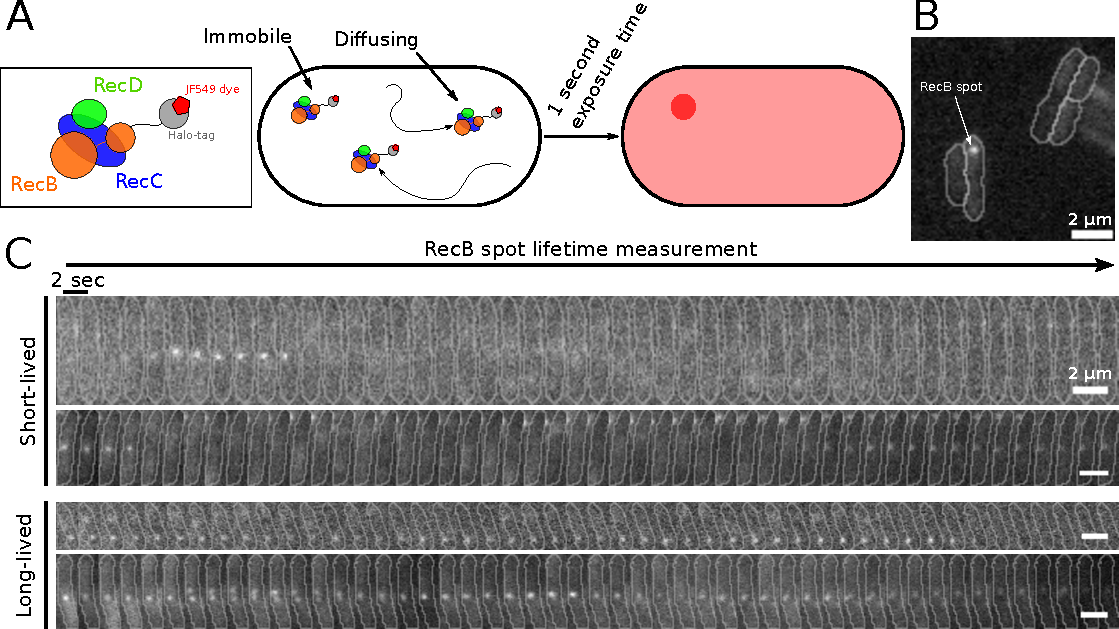
\includegraphics[width=.45\textwidth]{Figures/Fig1_Exp_principle.pdf}
    \caption{Detecting RecB binding to DSBs. \textbf{(A)} Scheme of our experimental protocol. The RecB subunit of the RecBCD complex is fused to a Halo-tag, bound by the JF549 fluorescent dye\cite{Lepore2019a, Lepore2023}. A long exposure time (1 sec) makes diffusing molecules appear as diffuse signal in the cell, while DNA-bound molecules are visible as bright, diffraction-limited spots. \textbf{(B)} Example image of a RecB spot (white arrow).}
    \label{Fig:exp_principle}
\end{figure}

\subsection*{RecB dissociation time is not affected by the concentration of cipro\-floxacin}

% RecB spot lifetime
Using the timelapse data, we built histograms of RecB spot lifetimes at the different ciprofloxacin concentrations (Figure \ref{Fig:lifetimes}B). In the absence of ciprofloxacin, a large majority of spots lasted less than 10 seconds. Under increasing ciprofloxacin concentrations, the distribution showed a clear shift towards longer-lived spots, with the histogram at 20 and 30 ng/ml ciprofloxacin displaying a clear "tail" of long-lived events ($>$ 10 sec). Fitting these histograms with a mono-exponential decay model ($y = a.e^{-k.t}$) did not match the experimental data accurately (Supp. Figure \ref{SIFig:monoexp_fits}). In particular, it did not account for the tail of longer-lived spots that formed at high ciprofloxacin concentrations. Fitting with a bi-exponential decay model ($y = a_1.e^{-k_1.t} + a_2.e^{-k_2.t}$) accounted better for the longer-lived RecB spots (Figure \ref{Fig:lifetimes}B). The bi-exponential fit outlined two populations of spots with different lifetimes: a short-lived one, with average lifetimes ranging from 1.4 to 1.7 sec, and a longer-lived one, with average lifetimes ranging from 10 to 14 sec (Table \ref{tab:fit_results}). Even though the short-lived spots always represented a majority of events (over 90\% of the spots), the proportion of long-lived spots tended to increase under higher ciprofloxacin exposure (from 1.4 $\pm$ 0.3\% at 3 ng/ml ciprofloxacin to 5.5 $\pm$ 1.4\% at 30 ng/ml ciprofloxacin).

\begin{figure*}[htbp]
    \centering
    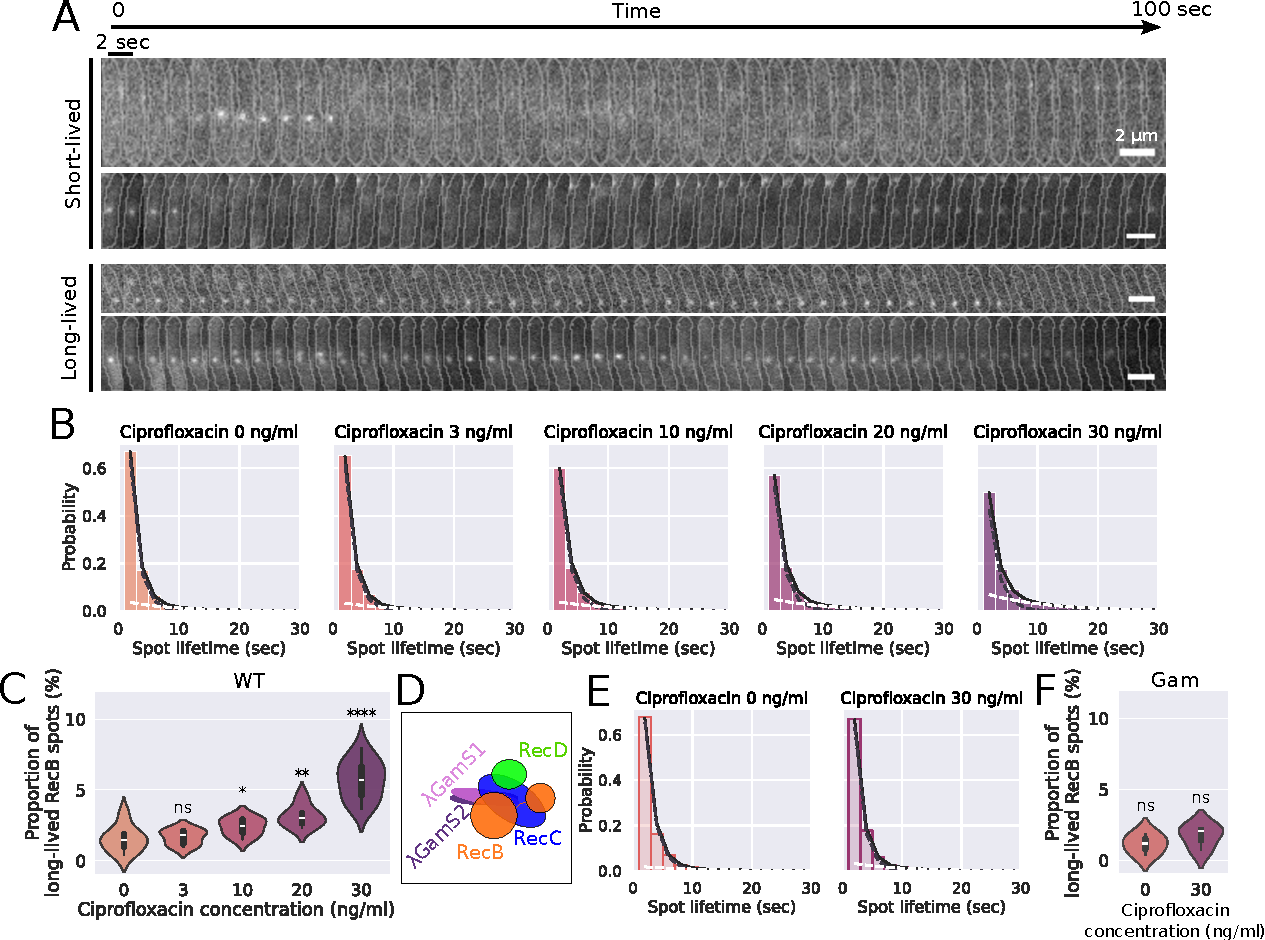
\includegraphics[width=.8\textwidth]{Figures/Fig2_RecB_lifetime.pdf}
    \caption{RecB lifetime on DNA under ciprofloxacin exposure. \textbf{(A)} Example kymographs (2 sec interval, 100 sec total) of cells containing short- and long-lived RecB spots. \textbf{(B)} RecB spot lifetime histograms at 0, 3, 10, 20 and 30 ng/ml ciprofloxacin (bars), fitted with a bi-exponential decay model (black line, fit components showed as dashed lines). \ncells{66,764}. \nspots{170,138}. \textbf{(C)} RecB spot lifetime histograms (bars) for cells over-expressing the Gam protein, fitted with a bi-exponential decay model (black line, fit components showed as dashed lines). \ncells{8,812}. \nspots{18,698}. \textbf{(D)} Probability of a spot corresponding to a DNA-bound RecB molecule, for cells over-expressing the Gam protein. Black dots show averages for individual datasets, the black line is the average between them, and the red dashed line shows the smallest lifetime at which RecB spots have 95\% probability to be DNA-bound. \ncells{8,812}. \nspots{18,698}.}
    \label{Fig:lifetimes}
\end{figure*}

\begin{table}[htbp]
    \centering
    \caption{Parameters derived from the spot lifetime histogram fits (Figures \ref{Fig:lifetimes}B and \ref{Fig:lifetimes}C). The lifetime was calculated as the inverse of the fitted dissociation rate. Values are given as the median $\pm$ standard deviation over at least 3 independent datasets. \ncells{66,764}. \nspots{170,138}}
    \begin{tabular}{lllll}
        \toprule
        &  &  & \makecell{Lifetime\\(sec)} & \makecell{Population\\(\%)} \\
        Strain & \makecell{Cipro.} & Type &  &  \\
        \midrule
        \multirow[t]{10}{*}{WT} & \multirow[t]{2}{*}{0 ng/ml} & Short & 1.4 $\pm$ 0.2 & 98.2 $\pm$ 1.0 \\
        &  & Long & 9.5 $\pm$ 9.7 & 1.8 $\pm$ 1.0 \\
        \cline{2-5}
        & \multirow[t]{2}{*}{3 ng/ml} & Short & 1.5 $\pm$ 0.1 & 98.6 $\pm$ 0.3 \\
         &  & Long & 10.5 $\pm$ 1.3 & 1.4 $\pm$ 0.3 \\
        \cline{2-5}
        & \multirow[t]{2}{*}{10 ng/ml} & Short & 1.7 $\pm$ 0.2 & 97.6 $\pm$ 0.6 \\
        &  & Long & 13.7 $\pm$ 2.3 & 2.4 $\pm$ 0.6 \\
        \cline{2-5}
        & \multirow[t]{2}{*}{20 ng/ml} & Short & 1.6 $\pm$ 0.2 & 96.6 $\pm$ 0.8 \\
        &  & Long & 11.8 $\pm$ 2.1 & 3.4 $\pm$ 0.8 \\
        \cline{2-5}
        & \multirow[t]{2}{*}{30 ng/ml} & Short & 1.7 $\pm$ 0.2 & 94.5 $\pm$ 1.4 \\
        &  & Long & 13.3 $\pm$ 2.2 & 5.5 $\pm$ 1.4 \\
        \midrule
        \multirow[t]{4}{*}{Gam} & \multirow[t]{2}{*}{0 ng/ml} & Short & 1.7 $\pm$ 0.2 & 99.2 $\pm$ 0.4 \\
        &  & Long & 15.5 $\pm$ 9.1 & 0.8 $\pm$ 0.4 \\
        \cline{2-5}
        & \multirow[t]{2}{*}{30 ng/ml} & Short & 1.5 $\pm$ 0.1 & 98.2 $\pm$ 0.9 \\
        & & Long & 8.2 $\pm$ 1.8 & 1.8 $\pm$ 0.9 \\
        \bottomrule
        \end{tabular}
    \label{tab:fit_results}
\end{table}

% Gam
To determine whether short- or long-lived spots resulted from RecB binding to DNA leading to SOS induction, we measured RecB spot lifetime in the presence and absence of ciprofloxacin while over-expressing the Gam protein of phage $\lambda$ from a plasmid. The Gam protein was previously shown to bind in place of DNA on the RecBCD complex\cite{Wilkinson2016}, and its overexpression is expected to abolish RecBCD binding to DSBs. Accordingly, cells that over-expressed Gam and were exposed to high ciprofloxacin (30 ng/ml) showed little elongation compared to cells that did not overexpress Gam (Supp. Figure \ref{SIFig:Gam_cell_length}), indicating that most cells did not induce the SOS response, due to the inability of the RecBCD-Gam complex to bind to DSBs and load RecA. The resulting RecB spot lifetimes showed a similar distribution to the one obtained in the absence of ciprofloxacin (Supp. Figure \ref{SIFig:Gam_RecB_lifetimes_vs_WT}). This was confirmed by fitting the histogram with our bi-exponential decay model (Figure \ref{Fig:lifetimes}C), which found a proportion of long-lived spots in the presence of 30 ng/ml ciprofloxacin (1.8 $\pm$ 0.9\%, Table \ref{tab:fit_results}) equivalent to wild-type cells that were not exposed to ciprofloxacin (1.8 $\pm$ 1\%). The residual amount of long-lived RecB spots in the presence of Gam could be due to residual DNA binding despite the presence of Gam. This residual binding could also be the cause for the small increase in cell length observed in Gam-expressing cells under 30 ng/ml ciprofloxacin (Supp. Figure \ref{SIFig:Gam_cell_length}). Since Gam overexpression prevents RecB binding to DNA ends, and specifically caused long-lived spots to disappear, we can conclude that long-lived spots correspond to RecB molecules that have bound to a DSB. Given that under Gam overexpression, 95\% of RecB spots were shorter than 10 sec (Figure \ref{Fig:lifetimes}D), we considered any spot with a lifetime over 10 sec to be a DNA-bound RecB molecule. The appearance of short-lived spots in the presence of Gam is likely due to a combination of short-lived DNA binding and slow, confined diffusion of the RecBCD-Gam-Halo complex (Supp. Note \ref{note:spurious_spots} and Supp. Figure \ref{SIFig:displacement_simul}). Therefore, spots that are visible for less than 10 seconds cannot be reliably assigned as either DNA-bound or not. However, the largely reduced cell elongation in the presence of Gam (Supp. Figure \ref{SIFig:Gam_cell_length}) indicates that short-lived spots do not trigger the SOS response.

Using the Gam protein allowed us to identify DNA-bound RecB molecules as the longer-lived population in our bi-exponential fits of the RecB spot lifetime histograms. We determined that when it processes a DSB, RecB stays bound to DNA for 10 to 15 seconds on average, regardless of the ciprofloxacin concentration (Table \ref{tab:fit_results}). This is consistent with processing of DSBs by RecBCD taking place independently of the presence of other DSBs in the cell. In addition, to test whether the duration of ciprofloxacin exposure had an effect on spot lifetimes, we performed separate fits at 15 min intervals (Supp. Figure \ref{SIFig:RecB_lifetimes_timepoints}). The RecB spot lifetimes obtained were consistent with those reported in Table \ref{tab:fit_results} (10-15 sec for long-lived spots, and 1.5-2 sec for short-lived spots), indicating that RecB binding was not affected by the duration of ciprofloxacin exposure.

\subsection*{RecB dissociation time is independent of RecA loading}

% Effect of ciprofloxacin exposure on the different mutants
Next, we wanted to test whether RecB dissociation from DNA was influenced by the following step in the repair process, the loading of RecA on DNA. Therefore, we imaged the \dreca\ and \geneteneighty\ mutants in the presence and absence of 30 ng/ml ciprofloxacin. Supp. Figure \ref{SIFig:mutants_bf} shows defocussed brightfield images of wild-type and mutant cells that were not exposed to ciprofloxacin, or exposed to 30 ng/ml ciprofloxacin for 60 min. Supp. Figure \ref{SIFig:mutants_cell_lengths} shows the average cell lengths for the different strains and ciprofloxacin exposure durations. As previously observed, wild-type cells show a clear response to exposure to 30 ng/ml ciprofloxacin, where the cell length increases significantly due to induction of the SOS response. In contrast to this, since the \dreca\ mutant is unable to form a RecA filament, it is also unable to induce the SOS response. Cell length therefore remains unchanged, even upon prolonged exposure to 30 ng/ml ciprofloxacin. In the absence of ciprofloxacin, the \geneteneighty\ mutant cells were slightly more elongated than wild-type cells. This matches our previous observations that this mutant has a higher baseline of SOS induction than wild-type cells in the absence of exogenous DNA damage\cite{Lepore2023}. Upon exposure to ciprofloxacin, the cell length of the \geneteneighty\ mutant increased, albeit slightly less on average than the wild-type's (Supp. Figure \ref{SIFig:mutants_cell_lengths}). This might be a reflection of \teneighty's inability to directly load RecA on the DNA, and the use of the alternative RecFOR pathway leading to different time dynamics of the SOS response\cite{Ivancic-Bace_2003,Lepore2023}.

% RecB binding time in the mutants
As for the wild-type strain, we imaged RecB, computed histograms of RecB spot lifetimes and fitted them with a bi-exponential decay model (Supp. Figure \ref{SIFig:mutants_biexp_fits}), from which we extracted the binding times of RecB on DNA (Table \ref{tab:fit_mutants}). In the \dreca\ mutant, the DNA-binding lifetime of RecB was similar to the wild-type ($\sim$12 sec), both in the presence and absence of ciprofloxacin. This suggests that RecA loading by RecBCD does not play a role in triggering the dissociation of wild-type RecBCD from DNA. In contrast, \teneighty\ stayed bound to DNA for longer on average than wild-type RecB ($\sim$16 to 19 sec). This could be due to the inability of \teneighty\ to digest the DNA it unwinds, making dissociation more challenging due to the DNA strands threading through the RecBCD complex.

% Table 2: RecB spot lifetime in the mutants
\begin{table}[htbp]
    \centering
    \caption{Parameters derived from the spot lifetime histogram fits for the \dreca\ and \geneteneighty\ strains (Supp. Figure \ref{SIFig:mutants_biexp_fits}). The lifetime was calculated as the inverse of the fitted dissociation rate. Values are given as the median $\pm$ standard deviation over at least 3 independent datasets. \ncells{56,131}. \nspots{177,646}.}
    \begin{tabular}{lllll}
        \toprule
        &  &  & \makecell{Lifetime\\(sec)} & \makecell{Population\\(\%)} \\
        Strain & Cipro. & Type &  &  \\
        \midrule
        \multirow[t]{4}{*}{\dreca} & \multirow[t]{2}{*}{0 ng/ml} & Short & 1.8 $\pm$ 0.2 & 96.6 $\pm$ 1.0 \\
        &  & Long & 13.0 $\pm$ 1.8 & 3.5 $\pm$ 1.0 \\
        \cline{2-5}
        & \multirow[t]{2}{*}{30 ng/ml} & Short & 2.1 $\pm$ 0.2 & 90.5 $\pm$ 3.4 \\
        &  & Long & 12.4 $\pm$ 3.5 & 9.5 $\pm$ 3.4 \\
        \cline{1-5} \cline{2-5}
        \multirow[t]{4}{*}{$recB_{1080}$} & \multirow[t]{2}{*}{0 ng/ml} & Short & 1.8 $\pm$ 0.2 & 97.4 $\pm$ 0.9 \\
        &  & Long & 16.7 $\pm$ 5.5 & 2.6 $\pm$ 0.9 \\
        \cline{2-5}
        & \multirow[t]{2}{*}{30 ng/ml} & Short & 2.1 $\pm$ 0.1 & 96.5 $\pm$ 0.7 \\
        &  & Long & 19.4 $\pm$ 7.1 & 3.5 $\pm$ 0.7 \\
        \bottomrule
    \end{tabular}
    \label{tab:fit_mutants}
\end{table}

% Part 2: Rate of recruitment of RecB on the DNA
\subsection*{RecB binding can be used to estimate the rate of DSB formation}

\begin{figure}[htbp]
    \centering
    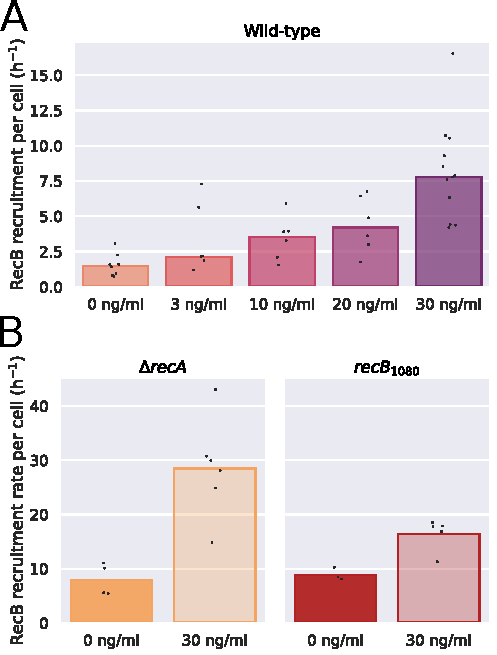
\includegraphics[width=.4\textwidth]{Figures/Fig3_RecB_recruitment.pdf}
    \caption{Recruitment of RecB to DSBs. \textbf{(A)} Recruitment rate of RecB on DNA per cell at different ciprofloxacin concentrations. Black points show averages for individual datasets, and bars the median value between them. \ncells{66,764}. \nspots{170,138}. \textbf{(B)} Recruitment rate of RecB on DNA per cell for the \dreca\ and \geneteneighty\ mutants. Black points show averages for individual datasets, and bars the median value between them. \ncells{23,540}. \nspots{99,891}.}
    \label{Fig:recruitment}
\end{figure}

% RecB recruitment in WT
Whereas the lifetime of RecB spots informs us on how long RecB stays bound to DNA, the rate of appearance of spots helps us estimate the rate of recruitment of RecB to DSBs under each DNA damage condition. To do so, we used the RecB spot lifetime histogram fits to estimate the total number of slow-dissociating spots per timelapse. Since we determined that the appearance of a slow-dissociating spot corresponds to the binding of RecB to a DSB, this allowed us to calculate the number of RecB recruitments to DSBs per cell per hour (Figure \ref{Fig:recruitment}A). We expect that the recruitment rate of RecB to DSBs gives a close estimate of the rate of formation of DSBs by ciprofloxacin (see discussion). We estimated that under endogenous damage or low ciprofloxacin concentrations, 1 to 2 RecB molecules are recruited to DSBs per hour on average. A previous study had estimated that 18\% of cells generated an endogenous DSB per cell cycle\cite{Sinha2018}. Considering the division time in our growth conditions (35 min), this would correspond to a rate of $\sim$0.3 DSBs per hour, a value roughly consistent with our own estimate. As expected, the recruitment rate of RecB scaled with ciprofloxacin concentration, up to 8 RecB recruited to DNA per hour at 30 ng/ml. It has been reported that DSB repair from the point of RecBCD binding takes $\sim$15 min in \ecoli\cite{Wiktor2021}; therefore, it appears consistent that undergoing 8 DSBs per hour at 30 ng/ml ciprofloxacin (a concentration higher than the Minimum Inhibitory Concentration, MIC) will cause multiple DSBs to be repaired simultaneously, and be lethal to most cells.

% RecB recruitment in mutants
Estimating the recruitment rate of RecB to DNA provided additional insight into the dynamics of DSB processing in the \dreca\ and \geneteneighty\ mutants (Figure \ref{Fig:recruitment}B). In the \dreca\ mutant, the rate of recruitment of RecB to DSBs was increased compared to wild-type cells, both in the presence and absence of ciprofloxacin. As in both cases the rate of DSB formation is expected to be the same between the wild-type and the \dreca\ mutant, we can hypothesise that this higher rate of RecB recruitment to DNA is due to multiple recruitment events on the same original DSB that cannot be repaired. In the mutant cells, RecBCD processes the DNA, but the generated ssDNA cannot be coated with the RecA protein, and is therefore likely to be degraded by cellular endo- and exonucleases such as SbcCD and ExoI\cite{Zahradka2009}. Degradation of the ssDNA would lead to a blunting of the DNA end, hence creating a new substrate for RecBCD binding. This deleterious cycle was previously reported to occur in cells lacking the RecA protein, eventually leading to full chromosome degradation\cite{Capaldo1975,Skarstad1993}. In our experiment, it results in multiple recruitments of RecB to DNA for each DSB.

% Recruitment in RecB1080
In the \geneteneighty\ mutant, RecB recruitment is higher than in WT cells, but equivalent (in the absence of ciprofloxacin) or lower (in the presence of 30 ng/ml ciprofloxacin) to the level of RecB recruitment in the \dreca\ mutant (Figure \ref{Fig:recruitment}B). Upon DSB recognition, \teneighty\ unwinds DNA without digesting it, and dissociates $\sim$1.5 times slower than wild-type RecB (Tables \ref{tab:fit_results} and \ref{tab:fit_mutants}). After RecBCD dissociation, we expect two competing pathways to take place. Either (i) the unwound ssDNA is digested by cellular endo- and exonucleases, creating a new RecBCD substrate; or (ii) RecFOR displaces the SSB (Single-Strand DNA-Binding) protein and promotes RecA loading, allowing DNA repair by homologous recombination to proceed\cite{Ivancic-Bace_2003}. As a result, \teneighty\ can be recruited on DNA several times for each DSB (similarly to the \dreca\ mutant), but the cycle of re-recruitment can be broken by the action of RecFOR.

% Part 3: Imaging RecA foci and filaments
\subsection*{Ciprofloxacin exposure induces formation of RecA filaments and nucleoid compaction}

During DSB processing, RecBCD facilitates the loading of the RecA protein on single-stranded DNA. To broaden our view of the repair process downstream of RecBCD, we imaged a tandem fusion of RecA with the fluorescent protein SYFP2 which was previously shown to preserve RecA functionality\cite{Wiktor2021}. Based on the fluorescence distribution in the cells (Supp. Figure \ref{SIFig:reca_structures}A), we identified three states of RecA: diffuse, forming a bright focus, or forming an elongated filament, which matches previous \emph{in-vivo} observations of RecA\cite{Wiktor2021}. Because of the large diversity of shapes observed, especially for RecA filaments, the detection of RecA structures by rule-based algorithms was challenging. Therefore, we designed and trained a deep-learning algorithm capable of classifying individual cells based on the three types of spatial distributions cited above (Supp. Figures \ref{SIFig:object_class} and \ref{SIFig:reca_structures}B). In cells that were not exposed to ciprofloxacin, the RecA-associated fluorescence was mostly diffuse, and occasionally formed a bright focus or filament. This is consistent with the expectation that RecA diffuses freely in the cell in the absence of DNA damage, and only polymerises on DNA in the event of an endogenous DSB. After one hour of exposure, the proportion of cells that contained a RecA filament had increased to $\sim$40\% at 20 ng/ml ciprofloxacin, and $\sim$60\% at 30 ng/ml. RecA foci on the other hand formed quickly following ciprofloxacin exposure (present in $\sim$40\% of the cells after 15 min of exposure to 30 ng/ml ciprofloxacin) and came back to endogenous damage level after $\sim$1 hour. Taken together, these results show that RecA foci are transient structures in the repair process that do not accumulate under high DNA damage, whereas RecA filaments accumulate under constant exposure to ciprofloxacin (see Discussion).

% Part 4: Colocalisation of RecB with the nucleoid
\subsection*{DNA-bound RecB colocalises with the bacterial nucleoid}

\begin{figure*}[htbp]
    \centering
    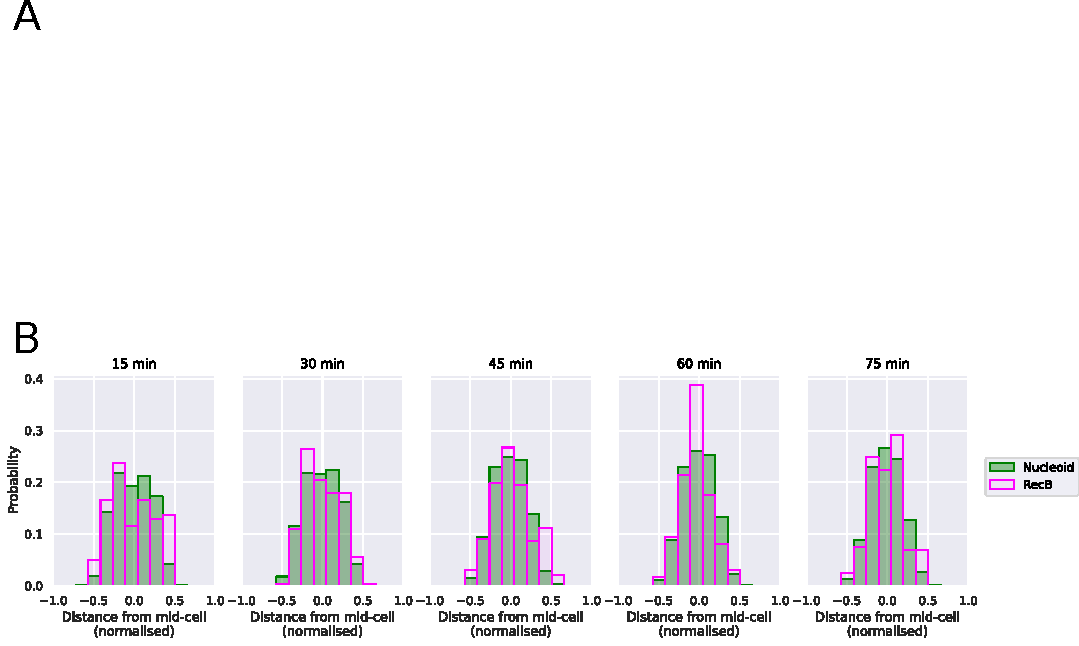
\includegraphics[width=.8\textwidth]{Figures/Fig4_nucleoid.pdf}
    \caption{Colocalisation of RecB spots with the bacterial nucleoid. \textbf{(A)} Representative images of cells (segmented outline in grey) showing the nucleoid (green) and RecB-associated fluorescence (magenta). RecB spots (indicated by arrows) are located in close proximity to the nucleoid. \textbf{(B)} Overlay of nucleoid density (green area) and position of DNA-bound RecB molecules (magenta bars) along the cell's long axis, for different ciprofloxacin concentrations (0 to 30 ng/ml). \ncells{24,014}. \nspots{79,969}. \nnucl{31,441}. \textbf{(C)} Representative overlay images of RecB-associated fluorescence (magenta) and the bacterial nucleoid (green) in the \dreca\ and \geneteneighty\ mutants. Segmented cell outline shown in grey. \textbf{(D)} Overlay of nucleoid density (green area) and position of DNA-bound RecB molecules (magenta bars) along the cell's long axis for the \dreca\ and \geneteneighty\ mutants at 0 and 30 ng/ml ciprofloxacin. \ncells{7,804}. \nspots{36,595}. \nnucl{11,215}.}
    \label{Fig:nucleoid}
\end{figure*}

% Nucleoid imaging
RecA loading on ssDNA triggers the SOS response, which inhibits cell division, leading to cell filamentation. Previous studies have reported that the SOS response also triggers compaction of the bacterial nucleoid\cite{Odsbu2014}. To see if this was the case for breaks induced by ciprofloxacin in our experimental conditions, we stained DNA using the Sytox Green dye. The use of a green dye allowed us to concomitantly image RecB, and to correlate the position of DNA-bound RecB molecules (defined as RecB spots with a lifetime $>$10 sec, see Figure \ref{Fig:lifetimes}D) with that of the nucleoid. Figure \ref{Fig:nucleoid}A shows representative images of the nucleoid and DNA-bound RecB after 60 minutes of exposure to different concentrations of ciprofloxacin. In untreated cells, the nucleoid was often observed to be bi-lobed, consistently with our previous observations\cite{Lepore2023}. After exposure to ciprofloxacin, the cells appeared elongated, and the nucleoid was often compacted in the centre of the cell. Due to nucleoid compaction, the total fraction of the cell occupied by the nucleoid decreased, from 40\% on average in untreated cells to 31\% in cells exposed to 30 ng/ml of ciprofloxacin for an hour (Supp. Figure \ref{SIFig:nucleoid_compaction}). In addition to the compaction, we observed that nucleoids were increasingly centred and the cells elongated upon increasing exposure to ciprofloxacin (in time and concentration), as shown in Supp. Figure \ref{SIFig:nucleoid_position}.

% Correlation of nucleoid and RecB spots
Long-lived RecB spots were found in close proximity to the nucleoid (Figure \ref{Fig:nucleoid}A), which strengthens our interpretation that they are DNA-bound RecB molecules. Figure \ref{Fig:nucleoid}B shows the spatial distribution of DNA-bound RecB spots and the nucleoid density in the cell (Supp. Figure \ref{SIFig:recb_nucleoid_timepoints} shows the same data after different durations of ciprofloxacin exposure). Upon exposure to increasing ciprofloxacin concentrations, induction of the SOS response caused the cells to elongate significantly (from 3.1 $\pm$ 0.19µm on average in the absence of ciprofloxacin to 5.5 $\pm$ 0.71µm after 75 min of exposure to 30 ng/ml ciprofloxacin, Supp. Figure \ref{SIFig:Gam_cell_length}). Despite this, and due to compaction and centring, the nucleoid remained within $\sim$2 µm either side of the cell centre. The distribution of DNA-bound RecB molecules overlapped strongly with nucleoid density, indicating that as the nucleoid was compacted, newly formed DSBs triggered RecB recruitment at the centre of the cell, where the nucleoid was located. Furthermore, the close overlap of the distributions for DNA-bound RecB and nucleoid density strongly suggests that RecB binding occurs at random positions within the nucleoid, consistent with ciprofloxacin causing DSBs at random chromosomal locations.

\subsection*{Nucleoid compaction requires RecA loading}

The spatial distribution of nucleoid density and DNA-bound RecB was affected in the \dreca\ and \geneteneighty\ mutants (Figures \ref{Fig:nucleoid}C and \ref{Fig:nucleoid}D). In the \dreca\ mutant, exposure to ciprofloxacin did not trigger nucleoid compaction and centring as in wild-type cells. This confirmed that nucleoid compaction under ciprofloxacin exposure requires RecA loading, and most likely the induction of the SOS response. Despite the absence of compaction, the nucleoid occupied a smaller fraction of the cell in the \dreca\ mutant after exposure to ciprofloxacin (Supp. Figure \ref{SIFig:mutants_nucleoid_compaction}). This can be attributed to the progressive degradation of the bacterial chromosome by the repeated cycles of RecBCD binding (Figure \ref{Fig:recruitment}B).

In the \geneteneighty\ mutant, the nucleoid often formed irregular shapes and small segregated regions in the cell (Figure \ref{Fig:nucleoid}C). This disorganisation was especially visible in the presence of 30 ng/ml ciprofloxacin. Furthermore, in the \geneteneighty\ mutant the nucleoid did not undergo compaction within the 75 min of our experiment (Supp. Figure \ref{SIFig:mutants_nucleoid_compaction}). This might be a reflection of the less efficient RecA loading in this mutant, leading to different time dynamics of the SOS induction and either impaired or significantly delayed nucleoid compaction.

In both mutant strains, the localisation of DNA-bound RecB overlapped with the bacterial nucleoid (Figure \ref{Fig:nucleoid}D), indicating that RecB binding occurred at random positions within the nucleoid, similarly to the wild-type. In the \dreca\ mutant, addition of 30 ng/ml ciprofloxacin did not change the spatial distribution of nucleoid density or DNA-bound RecB. This result was expected, as \dreca\ cells were unable to induce the SOS response, and therefore did not undergo nucleoid compaction. In the \geneteneighty\ mutant in the absence of ciprofloxacin, both nucleoid density and DNA-bound RecB distributions were more centred than in wild-type cells. This is consistent with the \geneteneighty\ mutant having a higher baseline of SOS induction than wild-type cells, as reported in our previous work\cite{Lepore2023}, which would result in a more compacted nucleoid on average. The absence of change in the distribution of nucleoid density and DNA-bound RecB position in the \geneteneighty\ mutant upon exposure to ciprofloxacin reinforces the hypothesis that nucleoid compaction is impaired or delayed in this mutant.


\section*{Discussion}

% Main things to discuss:
% - RecB dissociation, non-implication of RecA...: OK
% - RecB recruitment in WT; link to Alessia's article
% - RecB recruitment in mutants (OK, add links to Alessia's article)
% - RecA: OK
% - Nucleoid stuff

\subsection*{RecB dissociation does not depend on RecA loading}
One of the main questions asked in this study was how long RecBCD stays bound to DNA following DSB recognition. We have been able to estimate that in wild-type \ecoli, RecB stays bound to DNA for 10 to 15 seconds on average (Table \ref{tab:fit_results}), independently of the concentration of ciprofloxacin. Given RecBCD's high processivity (digesting several kilobases of DNA before recognising a Chi-site) and its processing speed ($\sim$1.6 kb/s\cite{Wiktor2018}), we can reasonably expect that most of RecB's binding time is explained by its DNA degradation prior to Chi recognition, followed by rapid disassembly after Chi. This led us to ask whether RecB dissociation from DNA was triggered by its interaction with RecA. Imaging RecB in a \dreca\ mutant confirmed that this is not the case, and that RecB dissociation occurs independently of RecA loading (Table \ref{tab:fit_mutants}). We can hypothesise that RecBCD's conformational change upon Chi recognition induces a destabilisation of the complex, thereby greatly reducing its processivity, and resulting in dissociation shortly after Chi. Interestingly, the \geneteneighty\ mutant had a reduced dissociation rate, which highlights the importance of RecB's exonuclease activity in the process. It is possible that digestion of the unwound DNA strands is a pre-requisite for RecBCD dissociation, and that it is performed by other cellular exonucleases in the \geneteneighty\ mutant.

\subsection*{Using RecB as a marker to quantify DSB formation}
Given RecBCD's high affinity for DSBs \emph{in-vivo} and our ability to detect its binding to DNA, the system is a useful tool to detect the presence of DSBs in \ecoli. Our experiments allowed us to estimate the number of recruitment of RecB to DSBs per hour, under different ciprofloxacin concentrations (Figure \ref{Fig:recruitment}A), and in the \dreca\ and \geneteneighty\ mutants (Figure \ref{Fig:recruitment}B). In the wild-type, the general pathway for DSB repair suggests that RecBCD is recruited once per DSB (Figure \ref{Fig:pathways}). We can therefore reasonably expect that the observed number of RecB recruitments observed matches with the number of DSBs formed (1 to 8 per hour, depending on ciprofloxacin concentration). In the \dreca\ and \geneteneighty\ mutants however, the disruptions to the DSB repair pathway lead to multiple RecB recruitments per DSB. We are therefore not able to estimate the rate of DSB formation in these mutants.

It should be noted that ciprofloxacin is expected to produce double-sided DSBs, hence leading to two RecB recruitments per break. We did not take this into account in our estimation of the DSB formation rate, as it has been previously suggested that the two sides of a DSB are kept in close proximity during DNA repair\cite{Vickridge2017,Keyamura2019}, and our imaging setup would not allow us to separate two RecB spots located close together. Indeed, our timelapse images of RecB binding seldom show two spots next to each other, further supporting the idea that we are not able to resolve RecBCD binding to both sides of a DSB.

Overall, our experimental setup provides a useful tool to quantify the availability of free double-stranded DNA ends in wild-type \ecoli\ \emph{in-vivo}.

\subsection*{Multiple RecB recruitments per DSB in the $\mathbf{\Delta}$\emph{reca} and RecB$\mathbf{_{1080}}$ mutants}

% Model of RecB recruitment to DNA
\begin{figure*}[htbp]
    \centering
    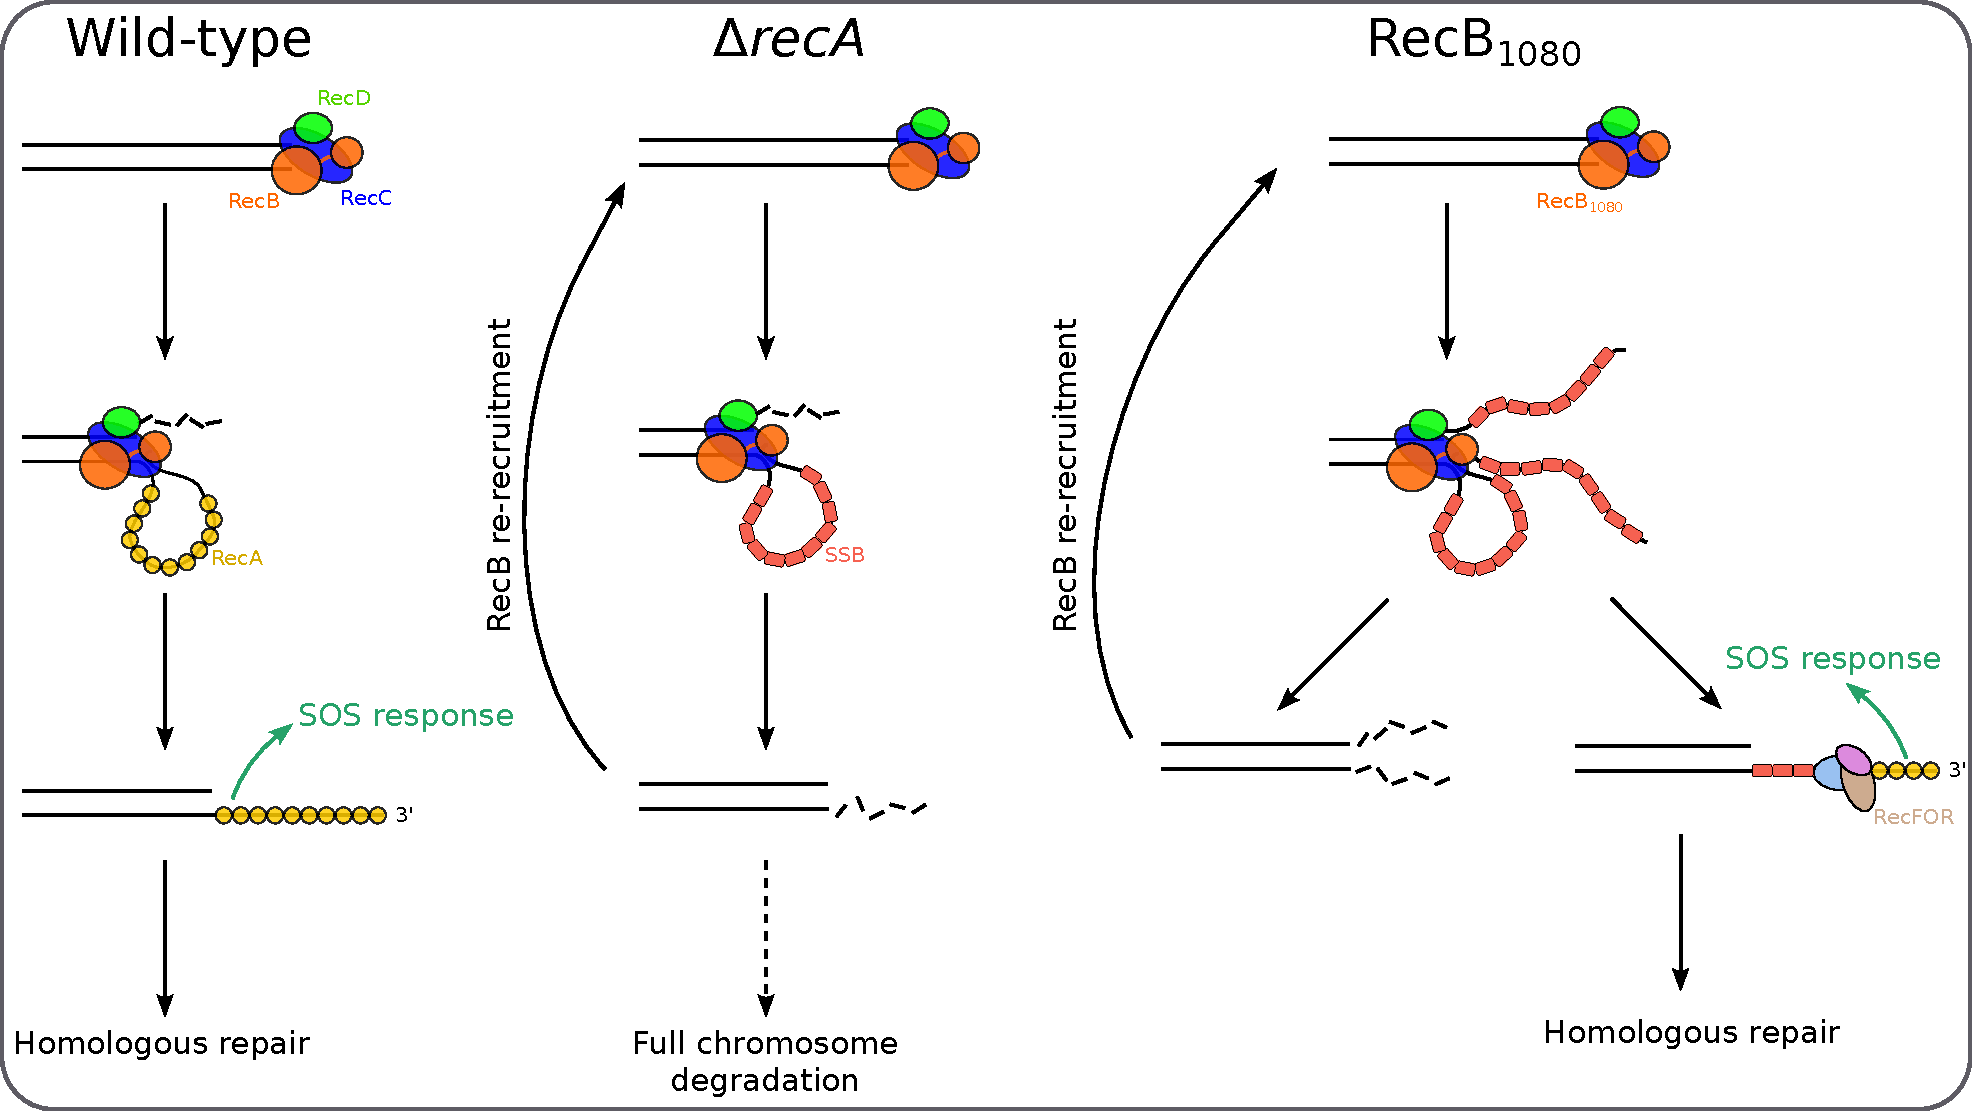
\includegraphics[width=\textwidth]{Figures/Fig_mutants_pathways.pdf}
    \caption{RecBCD recruitment pathways in wild-type \emph{E. coli}, \dreca\ and \geneteneighty\ mutants. \textbf{(Wild-type)} After DSB recognition, RecBCD degrades DNA until it recognises a Chi-site. It switches activity to create a 3' ssDNA overhang, and promotes RecA loading. The RecA-coated ssDNA can then be used for DNA repair by homologous recombination. \textbf{($\mathbf{\Delta}$reca)} In the absence of RecA, the 3' ssDNA is coated by SSB, and eventually digested by cellular nucleases. Blunting of the DNA end by digestion of the ssDNA creates a new substrate for binding of RecBCD. \textbf{(RecB$\mathbf{_{1080}}$)} Following DSB recognition, \teneighty\ unwinds DNA without digesting it. The unwound ssDNA can either be digested by nucleases, leading to a new blunt dsDNA end and RecBCD re-recruitment; or the RecFOR complex displaces SSB to load RecA, allowing DNA repair by homologous recombination to proceed.}
    \label{Fig:pathways}
\end{figure*}

Our observations of cell elongation (Supp. Figures \ref{SIFig:mutants_bf} and \ref{SIFig:mutants_cell_lengths}), RecB recruitment to DNA (Figure \ref{Fig:recruitment}), and nucleoid position (Figure \ref{Fig:nucleoid}) in the different mutant strains have led us to the model of RecB recruitment described in Figure \ref{Fig:pathways}. In wild-type cells, a DSB is recognised by RecBCD, which promotes RecA loading. The RecA filament triggers the SOS response, and is used for homology search and repair. In the \dreca\ mutant, the 3' ssDNA generated by RecBCD is first coated by SSB, and then degraded by the SbcCD and ExoI nucleases\cite{Zahradka2009}. This leads to blunting of the DNA end, creating a new substrate on which RecBCD can bind. This circle leads to multiple RecBCD recruitments per DSB, and eventually to full chromosome degradation. In the \geneteneighty\ mutant, RecBCD unwinds DNA without degrading it. After the ssDNA is coated with SSB, two competing pathways take place: either DNA degradation by SbcCD and ExoI leading to DNA-end blunting and re-recruitment of RecBCD, or displacement of SSB by RecFOR and loading of RecA, leading to SOS induction and homologous repair.

% Accumulation of RecA filaments at high cipro might be due to extensive DNA damage and unsuccessful homology search
\subsection*{Accumulation of RecA filaments under high DNA damage}
Under exposure to high ciprofloxacin concentrations (20-30 ng/ml), we observed an accumulation of cells that contained a RecA filament (Supp. Figures \ref{SIFig:reca_structures}A and \ref{SIFig:reca_structures}B). At these ciprofloxacin concentrations, we have determined that cells undergo frequent DSBs, leading to multiple recruitments of RecB to DNA over the course of the experiment (up to 8 per hour, Figure \ref{Fig:recruitment}A). Given RecBCD's high processivity\cite{Wiktor2018}, such a high number of RecB recruitments would likely result in several kilobases of DNA being digested at different chromosomal locations. Furthermore, it has been previously reported that DSB repair by RecBCD takes ~15 min from RecBCD binding to a DSB to completion of the repair\cite{Wiktor2021}. At a rate of 8 RecB recruitments per hour, it is likely that several DSBs would be processed simultaneously, resulting in fragmentation of the bacterial chromosome. If a homologous copy of the break site is not present in the cell, we expect that the repair process will stall at the homology search stage, after formation of the RecA filament, which is consistent with our observation that a large proportion of cells contain RecA filaments following exposure to over-MIC ciprofloxacin concentrations.



\begin{acknowledgements}
We would like to thank Prof. David Leach for insightful discussions on DNA repair in \emph{E. coli}. We thank Jean Ollion for the development of BACMMAN and its associated tools, as well as the image analysis support he provided. We thank Elise Darmon for discussing results, and reviewing the manuscript.
\end{acknowledgements}

\section*{Bibliography}
\bibliography{Bibliography}

\onecolumn
\newpage

%%%%%%%%%%%%%%%%%%%%%%%%%%%%%
% Supplementary Information %
%%%%%%%%%%%%%%%%%%%%%%%%%%%%%
\captionsetup*{format=largeformat}
\section{JF549 dye photobleaching kinetics}\label{note:dye_bleaching} 

In our approach to estimating RecB binding times to DSBs, the photostability of the fluorescent dye was of primary concern. Since we detect single molecules of RecB bound to DSBs, two main photophysical behaviours were liable to cause artefacts in our data:
\begin{enumerate}
    \item Photobleaching (an irreversible loss of fluorescence) would limit the maximum number of frames we can track a DSB-bound RecB for, and would artefactually reduce the fitted binding times since some fluorescent spots might disappear as a result of photobleaching rather than unbinding from DNA
    \item Blinking (a transient loss of fluorescence) could cause repeated disappearance and reappearance of single molecules, and, hence, bias the computed binding times and recruitment rates to DNA.\@
\end{enumerate}

To address these concerns, we computed ensemble-level photobleaching curves by integrating the total fluorescence signal from the cells (Supp. Fig.~\ref{SIFig:dye_bleaching}A). After 50 frames of laser exposure, a significant amount of photobleaching was noticeable (27\% $\pm$ 9 of the initial fluorescence remaining). The exact photobleaching rate of the dye in our experimental conditions can be estimated by fitting the photobleaching curve with an exponential decay function of the form $y=a.e^{-k.t}+b$ (with a the amplitude of the fit, k the bleaching rate, and b an offset to account for cellular auto-fluorescence). Since the bleaching rate is expected to mostly depend on experimental parameters that vary between but not within datasets (output laser power, HiLo angle), one bleaching rate was computed per dataset (Supp. Fig.~\ref{SIFig:dye_bleaching}B). The true RecB dissociation rates were computed by subtracting the corresponding bleaching rates from the fitted spot disappearance rates.

All experimental photobleaching curves were well-fitted by a mono-exponential decay function. If significant blinking of the dye was occurring, we would expect photobleaching curves to follow more complex kinetics~\cite{Thedie2017}. We therefore concluded that in our experimental conditions, the JF549 dye was not experiencing blinking, consistent with previous reports of the dye's outstanding photostability~\cite{Grimm2015}.

\section{Formation of RecB spots by the freely diffusing RecBCD-Halo-Gam complex}\label{note:spurious_spots}
In cells that overexpress the Gam protein, RecB is expected to be unable to bind DSBs. Even though Gam overexpression prevents the apparition of long-lived RecB spots under exposure to ciprofloxacin, short-lived RecB spots remain present (Figure~\ref{Fig:lifetimes}E, Supp. Figure~\ref{SIFig:Gam_RecB_lifetimes_vs_WT} and Supp. Table~\ref{SItab:fit_results}). To understand how RecB spots can be formed in the absence of DSB binding, we simulated the expected displacements of a RecBCD-Halo-Gam complex according to the distribution of single displacements for a random 2D walk:
\begin{equation}
    P(r) = \dfrac{r}{2D_i t}e^{-\dfrac{r^2}{4D_i t}}
\end{equation}

with $D_i$ the apparent diffusion coefficient, and $t$ the frame time. Our previous work found a diffusion coefficient for RecB-Halo of $\sim$1.5 \ums\ \cite{Lepore2025}. Assuming that the diffusion coefficient of the complex (that does not interact with DSBs) is proportional to the cube of the molecular weight, we expect a diffusion coefficient for the full RecBCD-Halo-Gam complex (386 kDa, 353 kDa without the Gam protein) of $\sim$1 \ums. The frame time in our experiments is 1 second, but it is likely that a molecule that would stay immobile for a fraction of that time would still be visible as a spot. Although calculating a precise value is challenging, we used a ballpark estimate of 500 ms (half our frame time) of a molecule being immobile to be detected as a spot in our experiment. Supp. Figure~\ref{SIFig:displacement_simul} shows the distribution of expected displacements under these parameters. Although most displacements would be too large to result in a bright fluorescent spot, a small fraction ($\sim$4\%) are smaller than 300 nm, and could create a spot. When factoring in the number of RecB molecules per cell [5 on average~\cite{Lepore2019a}] and the number of frames in our timelapse (50), this would result in $\sim$10 RecB spots per cell, on the same order of magnitude as the number of spots observed in our experiments in the presence of the Gam protein (4.1 $\pm$ 0.2, mean $\pm$ sem). Note that a single RecB molecule can form several spots over the length of the timelapse experiment.

\clearpage

\setlength\intextsep{40pt}

%% SUPPLEMENTARY FIGURES

% Strains table
\begin{supptable}[htbp]
    \centering
    \caption{List of bacterial strains used in this study}
    \begin{tabular}{lll}
        \toprule
        Name & Description & Reference\\
        \midrule
        MEK2623 & MG1655 \textit{recB::halotag recA::syfp2} & this work\\
        MEK2622 & MG1655 \textit{recB::halotag $\Delta$recA} & this work \\ % = AL133_1
        MEK716 & MG1655 \textit{recB1080::halotag} & this work \\ % = AL139_3
        MEK2324 & MG1655 \textit{recB1080::halotag HK022::psfiA-GFP} &~\cite{Lepore2025} \\
        MEK65 & MG1655 \textit{recB::halotag} &~\cite{Lepore2019a} \\
        MEK2629 & MG1655 \textit{recB::halotag pBad::GamL} & this work \\ % = AL119
        DL654 & MG1655 \textit{$\Delta$recA} &~\cite{Wertman1986} \\
        \bottomrule
    \end{tabular}\label{SItab:strains}
\end{supptable}

% Plasmids table
\begin{supptable}[htbp]
    \centering
    \caption{List of bacterial plasmids used in this study}
    \begin{tabular}{lll}
        \toprule
        Name & Description & Reference\\
        \midrule
        pSF1 & Expression of HaloTag under the control of the pBAD promoter &~\cite{Lepore2019a} \\
        pDT6 & GamL inserted into pBAD322K by restriction cloning &~\cite{Wilkinson2016} \\
        \bottomrule
    \end{tabular}\label{SItab:plasmids}
\end{supptable}

% Acquisition parameters table
\begin{supptable}[htbp]
    \centering
    \caption{Acquisition parameters used for microscopy.}
    \begin{tabular}{lllllll}
        \toprule
        Channel & Illumination & Intensity & Exposure (ms) & EM gain & Images (interval) & Z-stack\\
        \midrule
        Brightfield & Lamp & NA & 30 & 0 & 1 & 16 slices, 0.2 µm step\\
        JF549 & 561-nm & 2 mW & 1000 & 150 & 50 (2 sec) & No\\
        SYFP2 & 488-nm & 2 mW & 50 & 100 & 50 (2sec) & No\\
        Sytox Green & 488-nm & 2 mW & 50 & 100 & 1 & No\\
        \bottomrule
    \end{tabular}\label{SItab:acquisition_channels}
\end{supptable}

% Akaike's Information Criteria (AIC) table
\begin{supptable}[htbp]
    \centering
    \caption{Akaike's Information Criteria (AIC) for mono- and bi-exponential decay fits of the RecB spot lifetime histograms. Lower values (in bold) show the most relevant model. Values are given as the mean $\pm$ standard deviation on all datasets. Diff.\ shows the difference in mean AIC value between the two models (negative values are in favour of the bi-exponential model).}
    \begin{tabular}{lllllll}
        \toprule
        Ciprofloxacin concentration (ng/ml) & AIC (mono-exponential fit) & AIC (bi-exponential fit) & Diff. \\
        \midrule
        0 ng/ml & -258.5 $\pm$ 117.0 & \textbf{-284.5} $\pm$ 140.1 & -26 \\
        3 ng/ml & -307.0 $\pm$ 36.6 & \textbf{-322.2} $\pm$ 42.3 & -15 \\
        10 ng/ml & -290.4 $\pm$ 48.3 & \textbf{-340.2} $\pm$ 75.3 & -50 \\
        20 ng/ml & -286.4 $\pm$ 45.0 & \textbf{-349.6} $\pm$ 49.1 & -63 \\
        30 ng/ml & -303.5 $\pm$ 40.3 & \textbf{-387.5} $\pm$ 62.0 & -84 \\
        \bottomrule
    \end{tabular}\label{SItab:AIC}
\end{supptable}

% Fit results (WT and Gam)
\begin{supptable}[htbp]
    \centering
    \caption{Parameters derived from the spot lifetime histogram fits (Figures~\ref{Fig:lifetimes}B and~\ref{Fig:lifetimes}C). The lifetime was calculated as the inverse of the fitted dissociation rate. Values are given as the median $\pm$ standard deviation over at least 3 independent datasets.\ \ncells{66,764}.\ \nspots{170,138}}
    \begin{tabular}{lllll}
        \toprule
        &  &  & \makecell{Lifetime\\(sec)} & \makecell{Population\\(\%)} \\
        Strain & \makecell{Cipro.} & Type &  &  \\
        \midrule
        \multirow[t]{10}{*}{WT} & \multirow[t]{2}{*}{0 ng/ml} & Short & 1.4 $\pm$ 0.2 & 98.2 $\pm$ 1.0 \\
        &  & Long & 9.5 $\pm$ 9.7 & 1.8 $\pm$ 1.0 \\
        \cline{2-5}
        & \multirow[t]{2}{*}{3 ng/ml} & Short & 1.5 $\pm$ 0.1 & 98.6 $\pm$ 0.3 \\
         &  & Long & 10.5 $\pm$ 1.3 & 1.4 $\pm$ 0.3 \\
        \cline{2-5}
        & \multirow[t]{2}{*}{10 ng/ml} & Short & 1.7 $\pm$ 0.2 & 97.6 $\pm$ 0.6 \\
        &  & Long & 13.7 $\pm$ 2.3 & 2.4 $\pm$ 0.6 \\
        \cline{2-5}
        & \multirow[t]{2}{*}{20 ng/ml} & Short & 1.6 $\pm$ 0.2 & 96.6 $\pm$ 0.8 \\
        &  & Long & 11.8 $\pm$ 2.1 & 3.4 $\pm$ 0.8 \\
        \cline{2-5}
        & \multirow[t]{2}{*}{30 ng/ml} & Short & 1.7 $\pm$ 0.2 & 94.5 $\pm$ 1.4 \\
        &  & Long & 13.3 $\pm$ 2.2 & 5.5 $\pm$ 1.4 \\
        \midrule
        \multirow[t]{4}{*}{Gam} & \multirow[t]{2}{*}{0 ng/ml} & Short & 1.7 $\pm$ 0.2 & 99.2 $\pm$ 0.4 \\
        &  & Long & 15.5 $\pm$ 9.1 & 0.8 $\pm$ 0.4 \\
        \cline{2-5}
        & \multirow[t]{2}{*}{30 ng/ml} & Short & 1.5 $\pm$ 0.1 & 98.2 $\pm$ 0.9 \\
        & & Long & 8.2 $\pm$ 1.8 & 1.8 $\pm$ 0.9 \\
        \bottomrule
        \end{tabular}\label{SItab:fit_results}
\end{supptable}

% Fit results (drecA and recB1080)
\begin{supptable}[htbp]
    \centering
    \caption{Parameters derived from the spot lifetime histogram fits for the \dreca\ and \geneteneighty\ strains (Supp. Figure~\ref{SIFig:mutants_biexp_fits}). The lifetime was calculated as the inverse of the fitted dissociation rate. Values are given as the median $\pm$ standard deviation over at least 3 independent datasets.\ \ncells{56,131}.\ \nspots{177,646}.}
    \begin{tabular}{lllll}
        \toprule
        &  &  & \makecell{Lifetime\\(sec)} & \makecell{Population\\(\%)} \\
        Strain & Cipro. & Type &  &  \\
        \midrule
        \multirow[t]{4}{*}{\dreca} & \multirow[t]{2}{*}{0 ng/ml} & Short & 1.8 $\pm$ 0.2 & 96.6 $\pm$ 1.0 \\
        &  & Long & 13.0 $\pm$ 1.8 & 3.5 $\pm$ 1.0 \\
        \cline{2-5}
        & \multirow[t]{2}{*}{30 ng/ml} & Short & 2.1 $\pm$ 0.2 & 90.5 $\pm$ 3.4 \\
        &  & Long & 12.4 $\pm$ 3.5 & 9.5 $\pm$ 3.4 \\
        \midrule
        \multirow[t]{4}{*}{$recB_{1080}$} & \multirow[t]{2}{*}{0 ng/ml} & Short & 1.8 $\pm$ 0.2 & 97.4 $\pm$ 0.9 \\
        &  & Long & 16.7 $\pm$ 5.5 & 2.6 $\pm$ 0.9 \\
        \cline{2-5}
        & \multirow[t]{2}{*}{30 ng/ml} & Short & 2.1 $\pm$ 0.1 & 96.5 $\pm$ 0.7 \\
        &  & Long & 19.4 $\pm$ 7.1 & 3.5 $\pm$ 0.7 \\
        \bottomrule
    \end{tabular}\label{tab:fit_mutants}
\end{supptable}

% Acquisition pattern
\begin{suppfigure*}[htbp]
    \begin{center}
    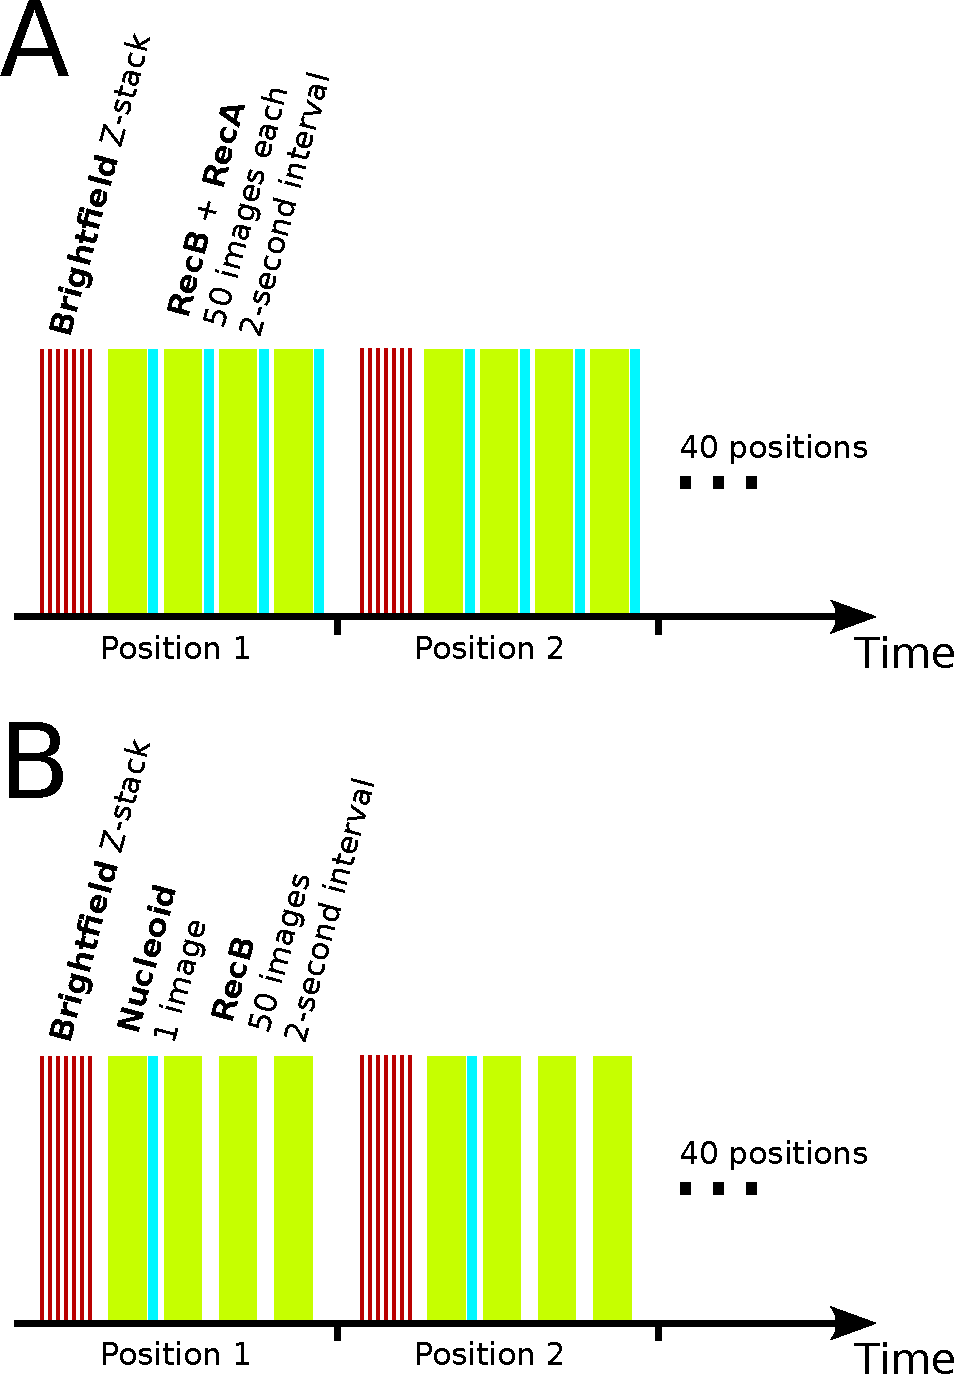
\includegraphics[width=.5\textwidth]{SI_Figures/Acquisition_pattern.pdf}
    \end{center}
    \caption{Acquisition patterns for microscopy experiments. \textbf{(A)} Acquisition pattern for experiments with brightfield, RecB (JF549) and RecA (SYFP2) channels. \textbf{(B)} Acquisition pattern for experiments with brightfield, RecB (JF549) and Nucleoid (Sytox Green) channels.}\label{SIFig:acquisition_pattern}
\end{suppfigure*}

% Photobleaching figure (curves + fitted rates)
\begin{suppfigure*}[htbp]
    \begin{center}
        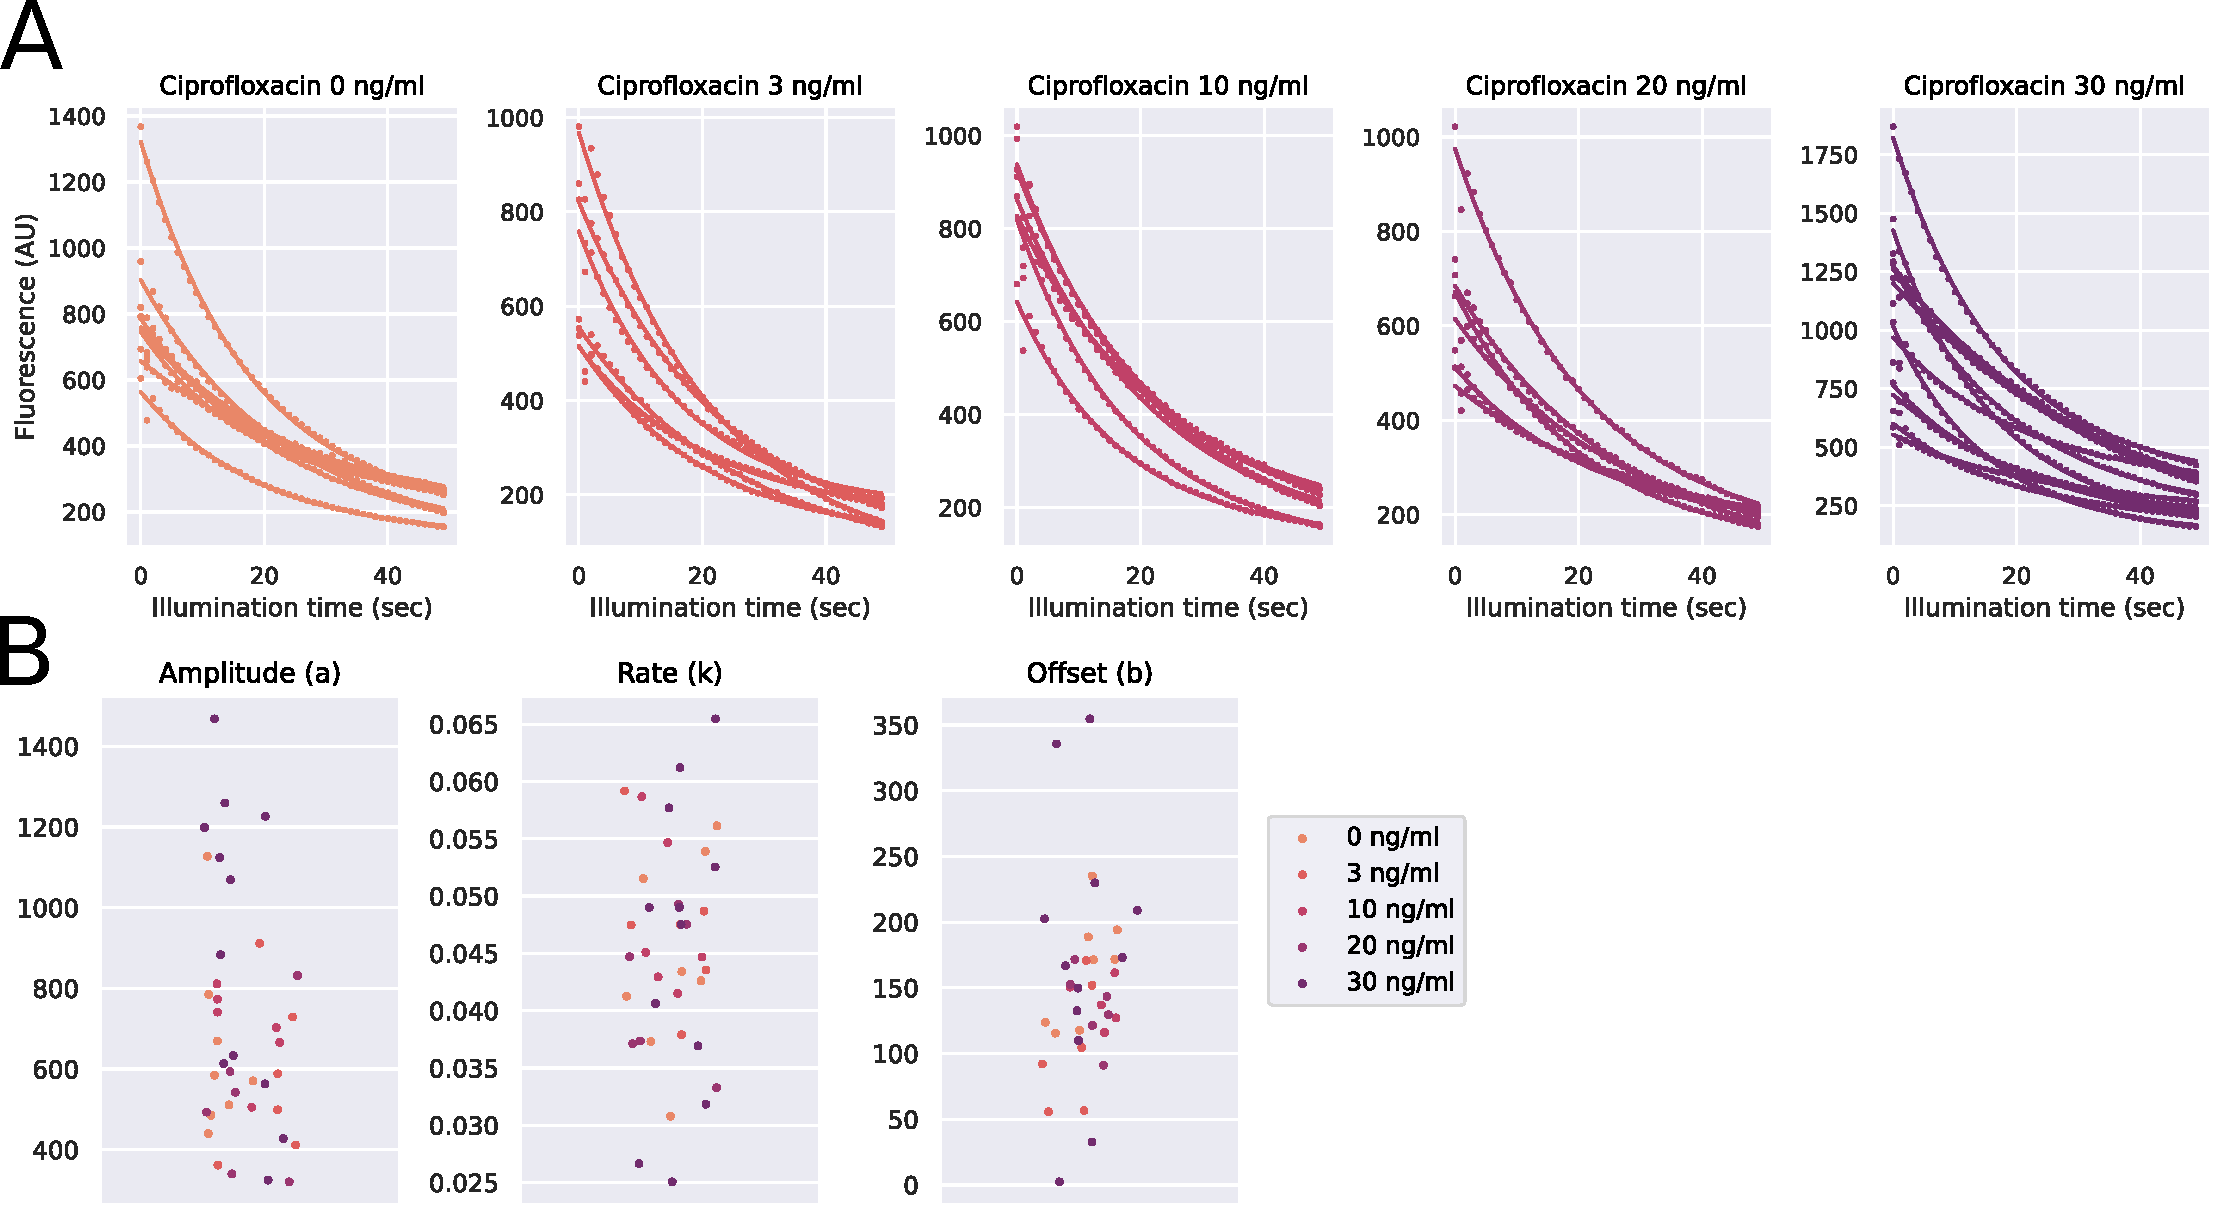
\includegraphics[width=\textwidth]{SI_Figures/SIFig_bleaching.pdf}
    \end{center}
    \caption{Ensemble-level photobleaching of the JF549 dye. \textbf{(A)} Average background-subtracted fluorescence for independent datasets (dots), overlaid with the photobleaching rate fit ($y=a.e^{-k.t}+b$, line).\ \ncells{66,764}. \textbf{(B)} Fitted model parameters for each dataset: amplitude (a), photobleaching rate (k) and offset (b).\ \ncells{66,764}.}\label{SIFig:dye_bleaching}
\end{suppfigure*}

% Data analysis pipeline
\begin{suppfigure*}[htbp]
    \begin{center}
        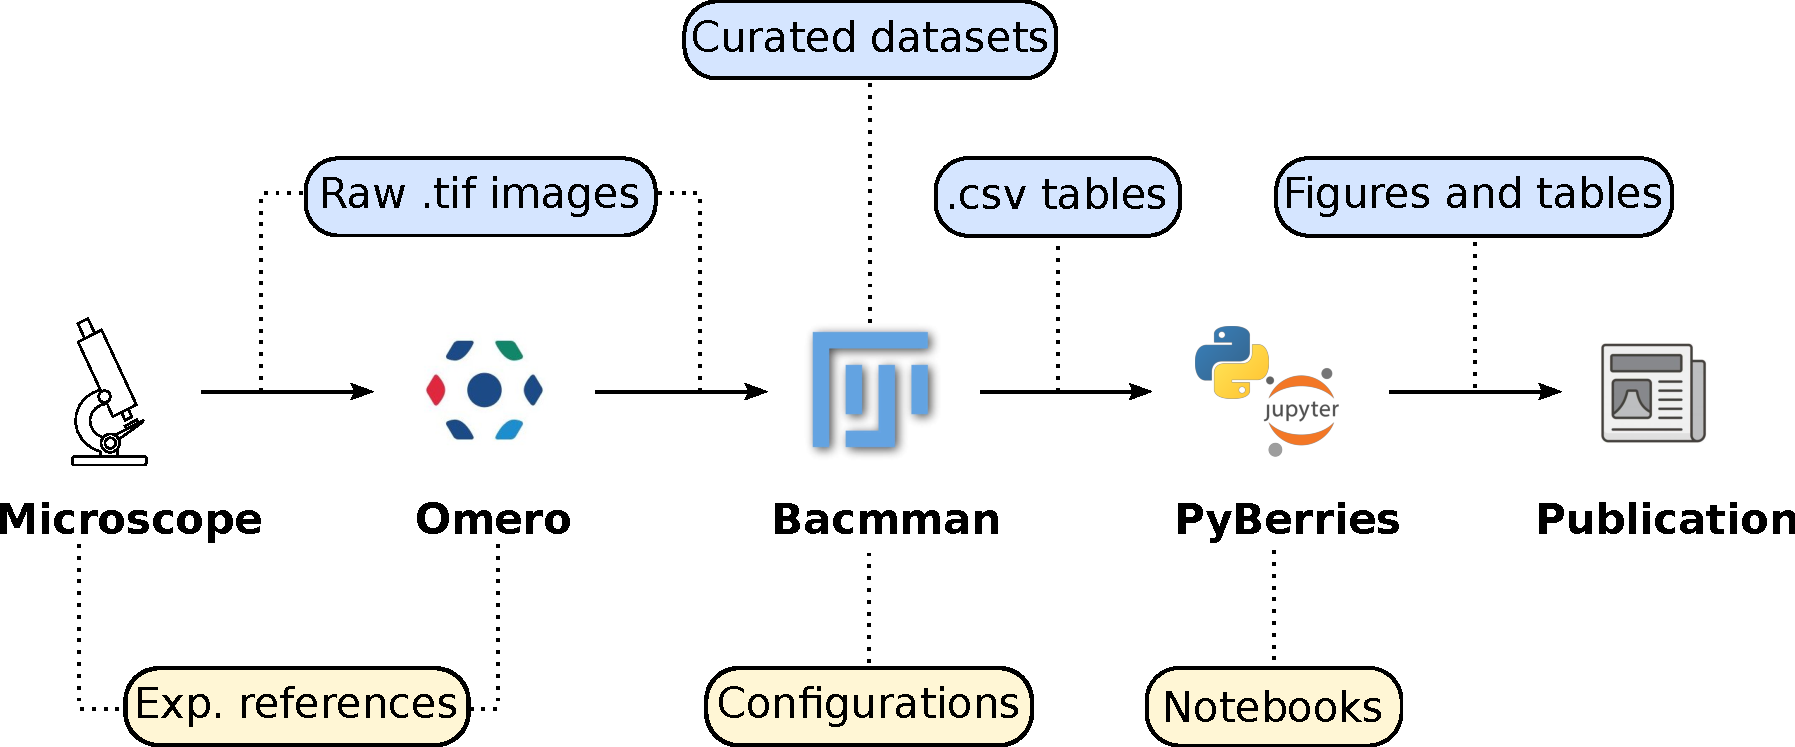
\includegraphics[width=\textwidth]{SI_Figures/Data_analysis_workflow.pdf}
    \end{center}
    \caption{Data storage and analysis pipeline used in this study. Blue labels indicate stored data and yellow labels indicate code and references that would allow reproducing the different analysis steps.}\label{SIFig:analysis_workflow}
\end{suppfigure*}

% Object classification workflow
\begin{suppfigure*}[htbp]
    \begin{center}
        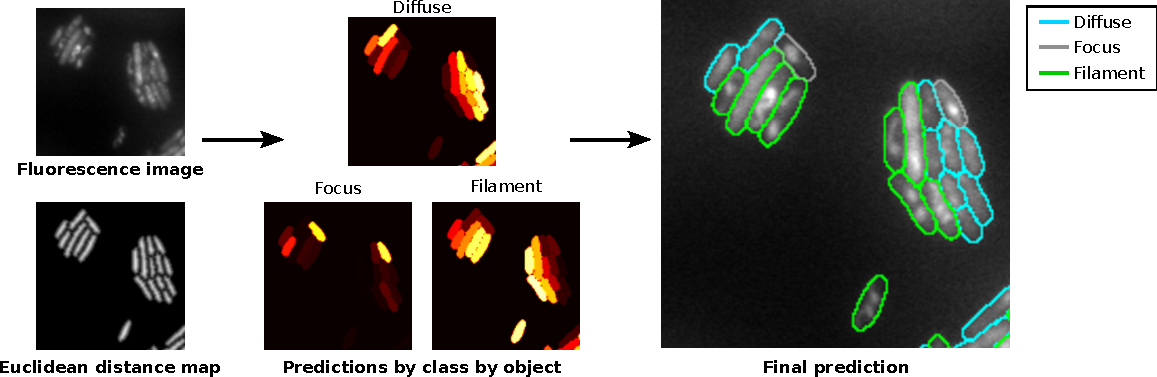
\includegraphics[width=\textwidth]{SI_Figures/ObjectClassifier.pdf}
    \end{center}
    \caption{Classification of cells according to the RecA structures they contain by our in-house Unet-based deep-learning network.}\label{SIFig:object_class}
\end{suppfigure*}

% Example image of freely diffusing halo-tag + JF549
\begin{suppfigure*}[htbp]
    \begin{center}
        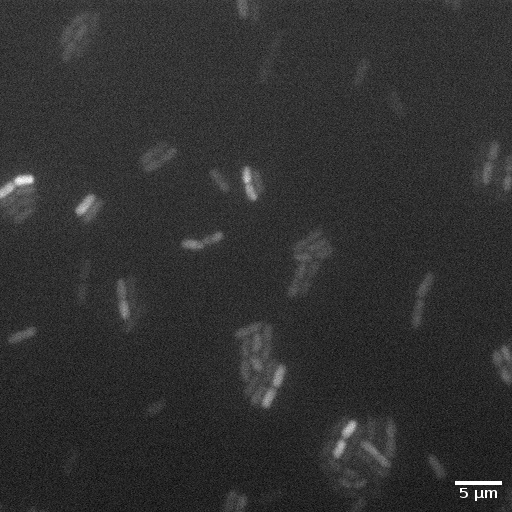
\includegraphics[width=.5\linewidth]{SI_Figures/Free_Halo_image.png}
    \end{center}
    \caption{Representative fluorescence image (1 second exposure time) of freely diffusing Halo-tag expressed from a pBAD plasmid (induced with 1\% w/v arabinose) in MG1655 \textit{E. coli} cells.}\label{SIFig:freehalo_image}
\end{suppfigure*}

% Example intensity time-traces for single RecB spots
\begin{suppfigure*}[htbp]
    \begin{center}
    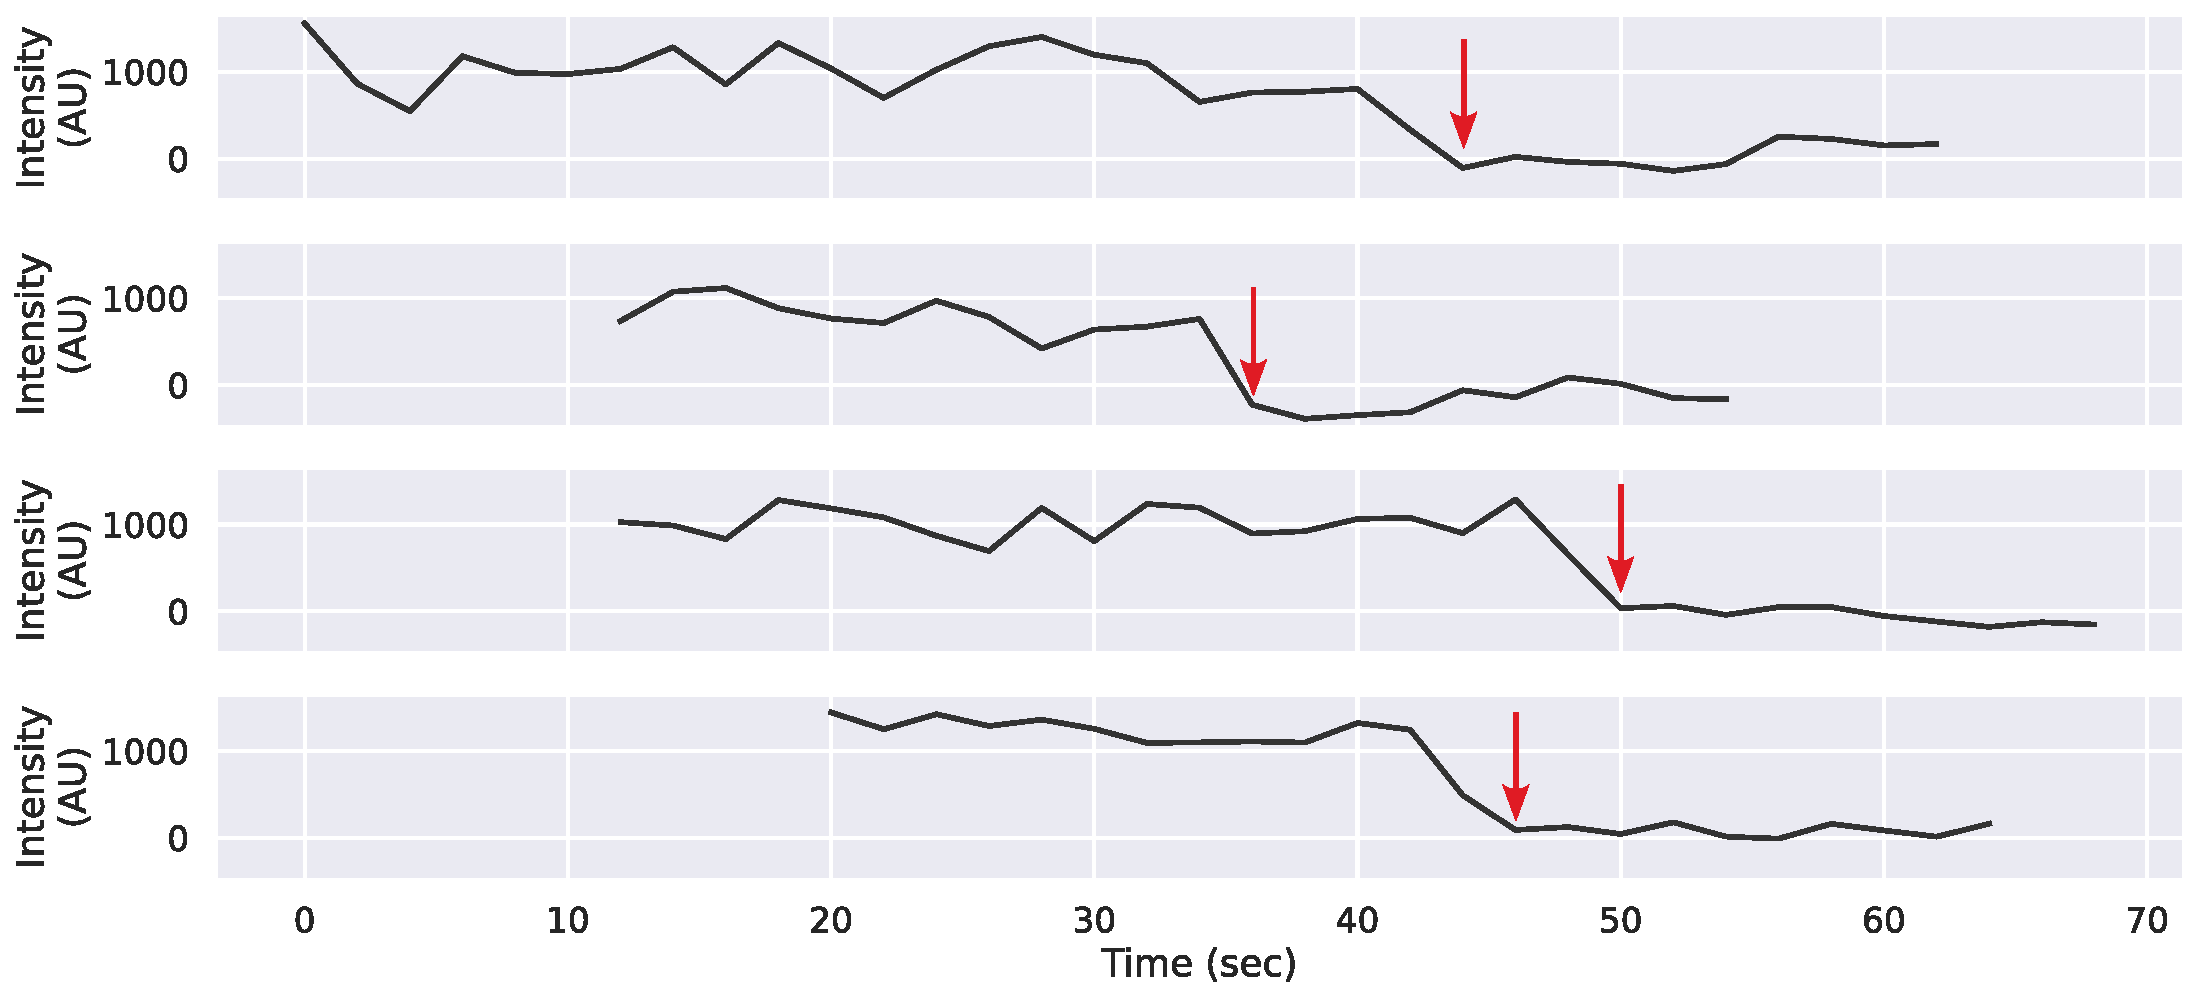
\includegraphics[width=.8\linewidth]{SI_Figures/SM_traces.pdf}
    \end{center}
    \caption{Representative background-subtracted intensity time traces (black lines) for single RecB spots, showing loss of intensity in a single step (red arrows).}\label{SIFig:SM_traces}
    \end{suppfigure*}

% Monoexponential fit of WT data, all cipro concentrations
\begin{suppfigure*}[htbp]
    \begin{center}
    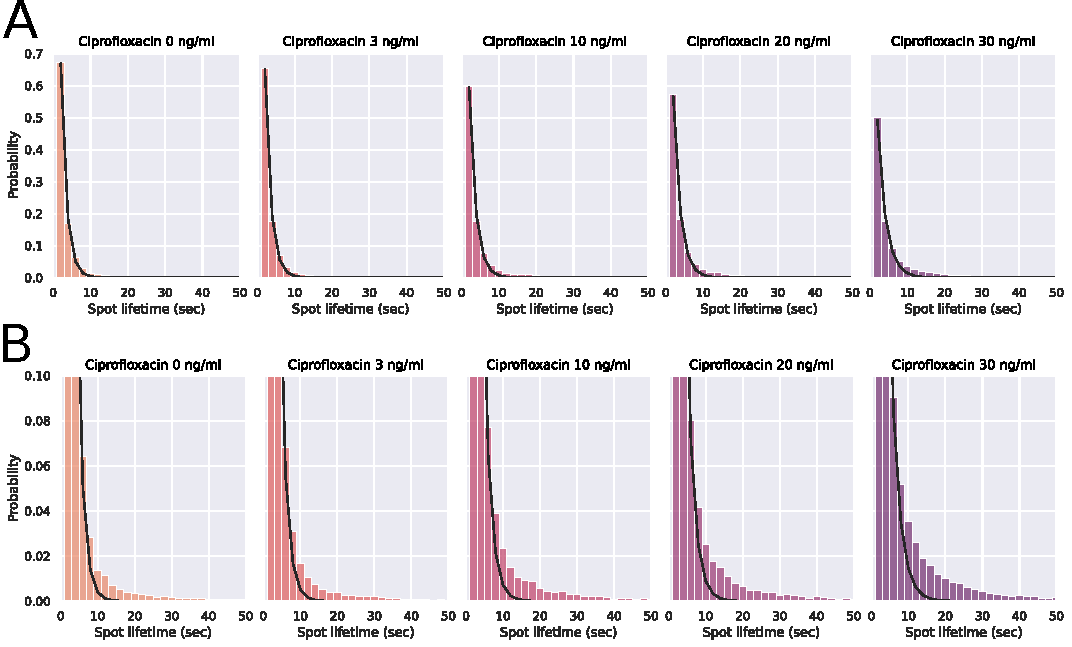
\includegraphics[width=\linewidth]{SI_Figures/Monoexp_fits_cipro.pdf}
    \end{center}
    \caption{\textbf{(A)} Histograms of RecB spot lifetime (bars) under exposure to ciprofloxacin, with overlaid mono-exponential decay fits ($y=a.e^{-k.t}$, black line).\ \ncells{66,764}.\ \nspots{170,138} \textbf{(B)} Zoom on the tails of histograms in (A).}\label{SIFig:monoexp_fits}
\end{suppfigure*}

% Cell length under Gam over-expression, 0 and 30 ng/mL cipro
\begin{suppfigure*}[htbp]
    \begin{center}
    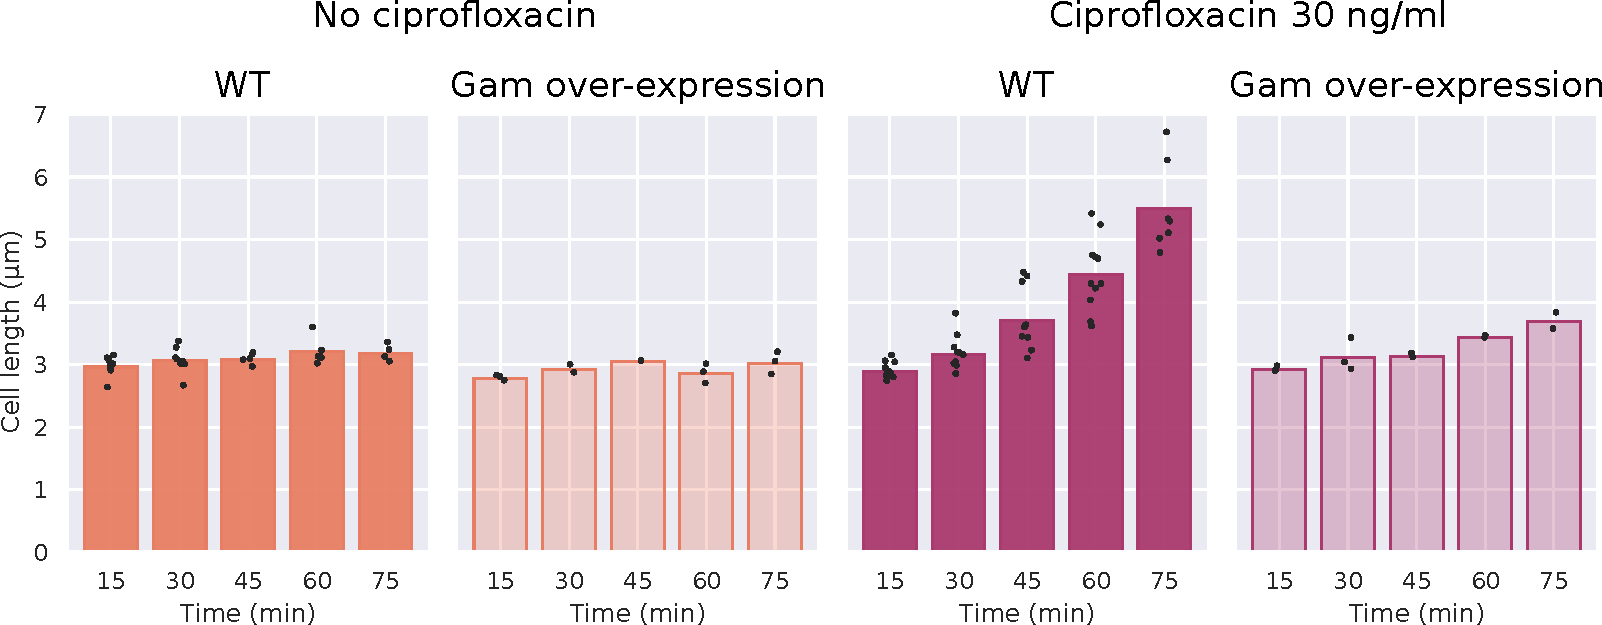
\includegraphics[width=\linewidth]{SI_Figures/Cell_length_Gam.pdf}
    \end{center}
    \caption{Average length of cells that over-express Gam or not (WT), under exposure to 0 or 30 ng/mL ciprofloxacin. Black dots show averages for indvidual datasets, and bars the average between them.\ \ncells{41,403}.}\label{SIFig:Gam_cell_length}
\end{suppfigure*}

% RecB spot lifetimes under Gam over-expression, 0 and 30 ng/mL cipro
\begin{suppfigure*}[htbp]
    \begin{center}
    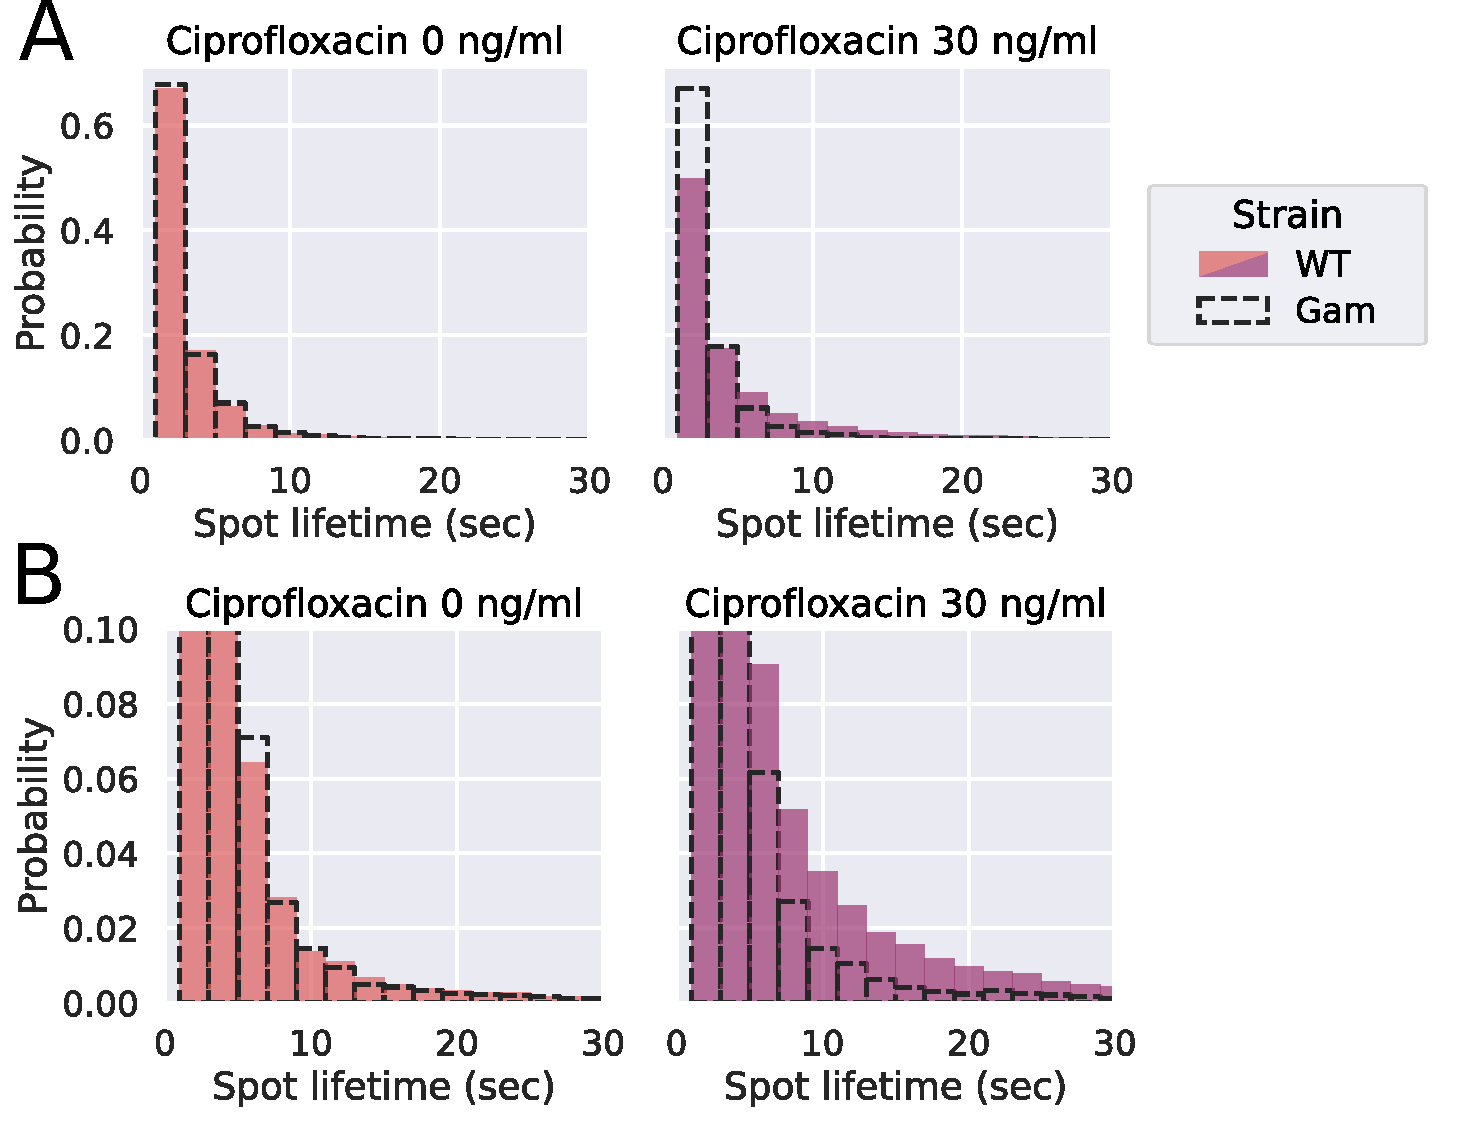
\includegraphics[width=0.75\linewidth]{SI_Figures/Gam_lifetimes_vs_WT.pdf}
    \end{center}
    \caption{\textbf{(A)} Histograms of RecB spot lifetimes for wild-type cells (coloured bars) and cells overexpressing Gam (dashes).\ \ncells{41,403}.\ \nspots{96,453} \textbf{(B)} Zoom on the tail of the histograms from (A).}\label{SIFig:Gam_RecB_lifetimes_vs_WT}
\end{suppfigure*}

% Probability for a spot to be DSB-bound depending on its lifetime
\begin{suppfigure*}[htbp]
    \begin{center}
        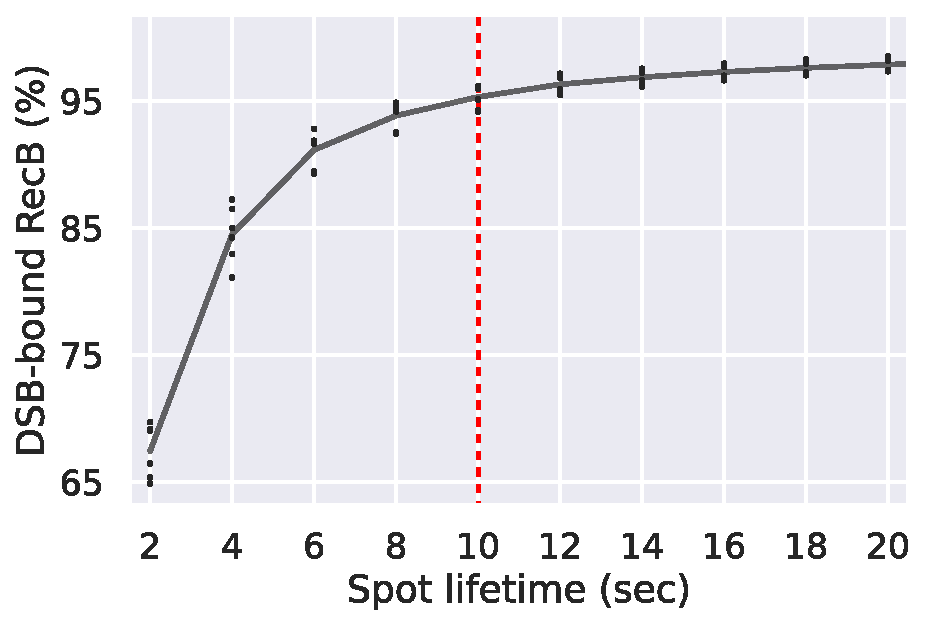
\includegraphics[width=.4\textwidth]{SI_Figures/Proba_DSB_bound.pdf}
    \end{center}
    \caption{Proportion of DSB-bound RecB molecules according to RecB spot lifetime. Black dots show averages for individual datasets; the black line is the average between them, and the red dashed line shows the smallest lifetime at which RecB spots have a 95\% probability of being DSB-bound.\ \ncells{8,812}.\ \nspots{18,698}.}\label{SIFig:proba_DSB_bound}
\end{suppfigure*}

% Displacements simulation
\begin{suppfigure*}[htbp]
    \begin{center}
        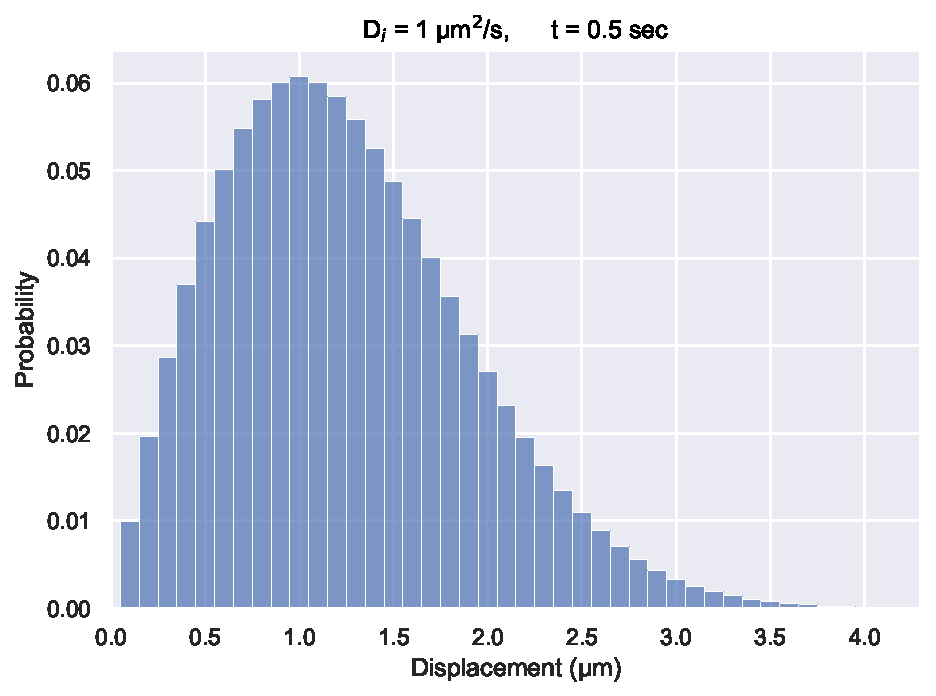
\includegraphics[width=.8\textwidth]{SI_Figures/Displacements_distribution.pdf}
    \end{center}
    \caption{Histogram of expected displacements for a molecule diffusing at 1 \ums\ over a 500 ms frame time.}\label{SIFig:displacement_simul}
\end{suppfigure*}

% Fitted RecB spot lifetimes at different durations of ciprofloxacin exposure
\begin{suppfigure*}[htbp]
    \begin{center}
        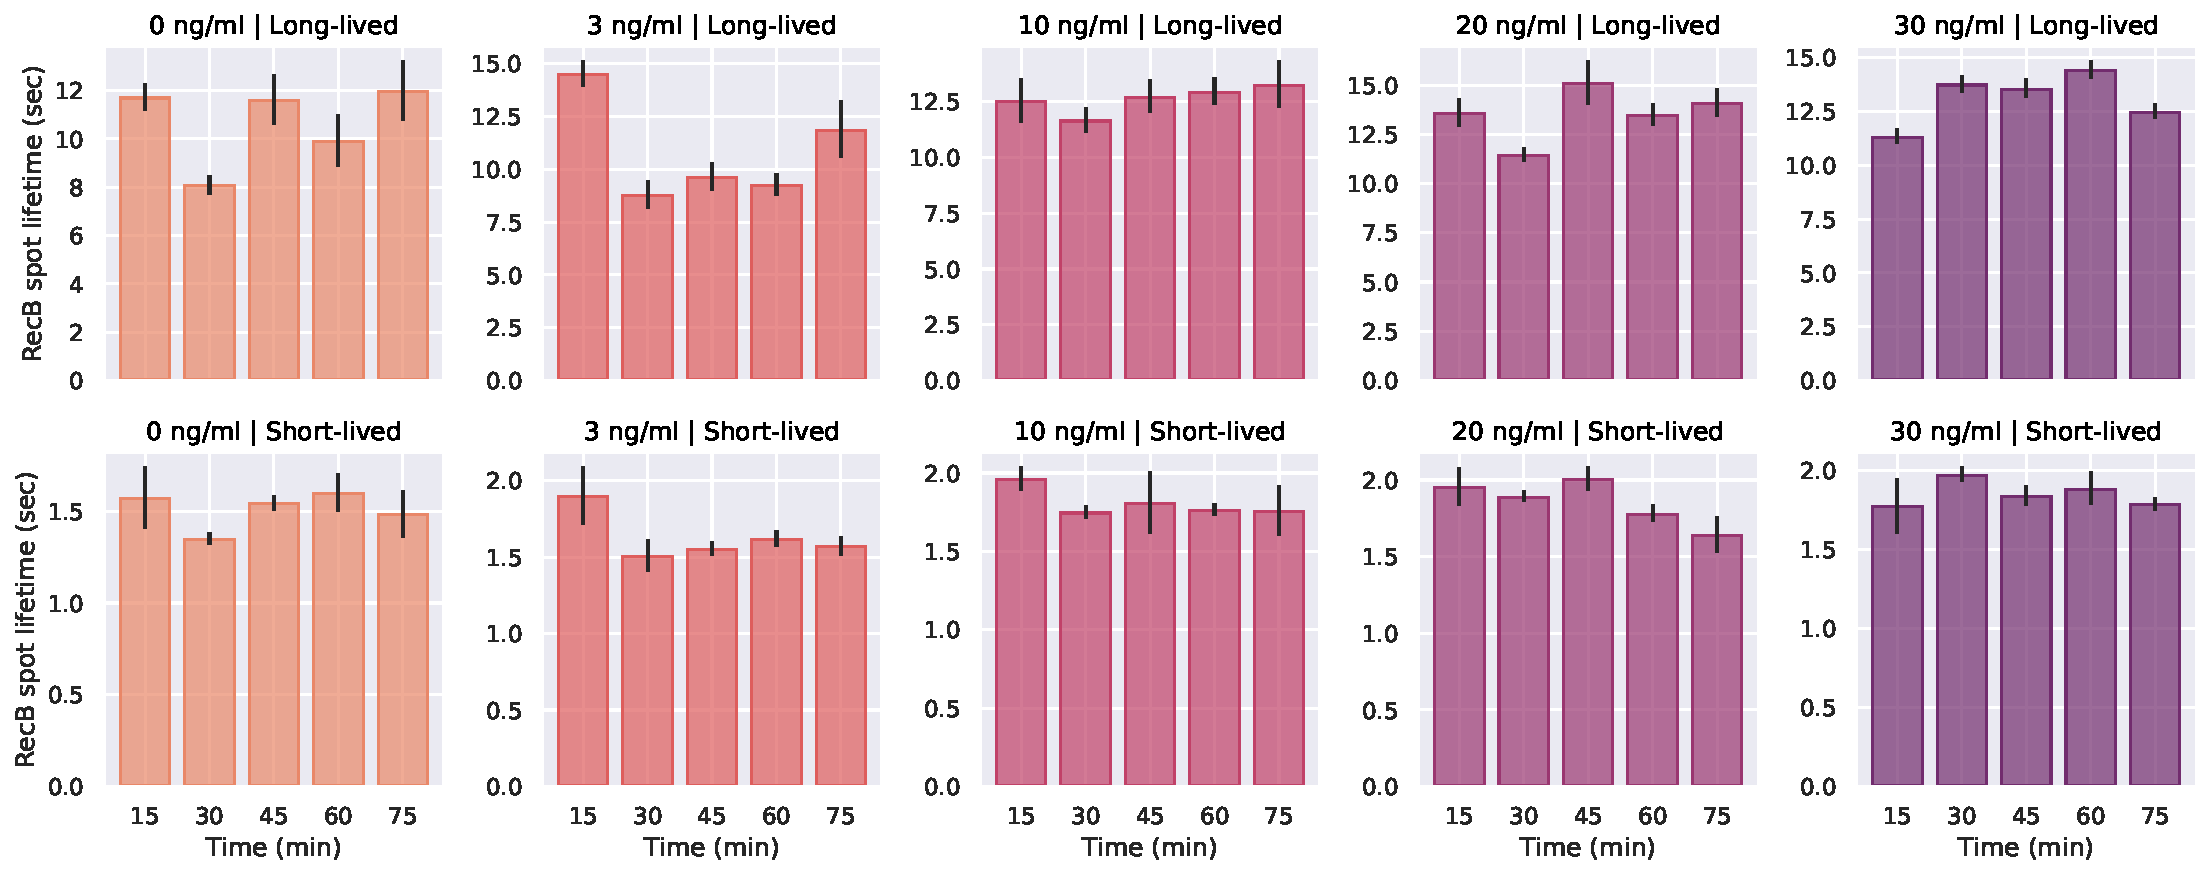
\includegraphics[width=.7\linewidth]{SI_Figures/RecB_lifetime_timepoints.pdf}
    \end{center}
    \caption{Fitted lifetimes of short- and long-lived RecB spots, following different durations of exposure to 30 ng/ml ciprofloxacin. Coloured bars represent the fitted lifetimes, and black strokes the standard error of the mean obtained by bootstrapping.\ \ncells{18,945}.\ \nspots{54,475}}\label{SIFig:RecB_lifetimes_timepoints}
    \end{suppfigure*}

% Mutants: RecB spot lifetime histogram bi-exp fits
\begin{suppfigure*}[htbp]
    \begin{center}
        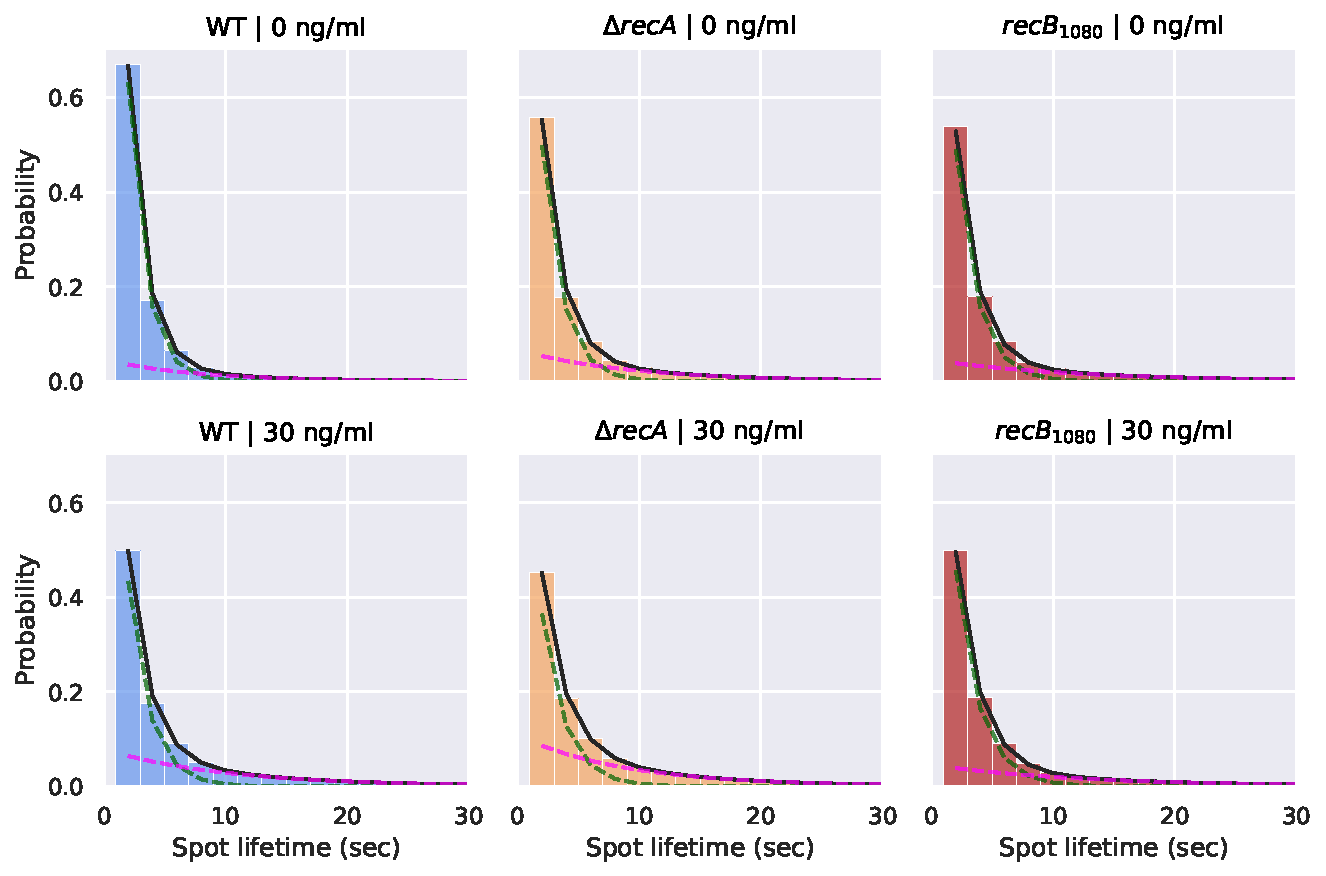
\includegraphics[width=.8\textwidth]{SI_Figures/Mutants_RecB_fits.pdf}
    \end{center}
    \caption{RecB spot lifetime histograms for wild-type (WT), \dreca\ and \geneteneighty\ mutants, at 0 and 30 ng/mL ciprofloxacin, fitted with a bi-exponential decay model (black line, fit components showed as dashed lines).\ \ncells{56,131}.\ \nspots{177,646}.}\label{SIFig:mutants_biexp_fits}
\end{suppfigure*}

% RecA structures
\begin{suppfigure*}[htbp]
    \begin{center}
    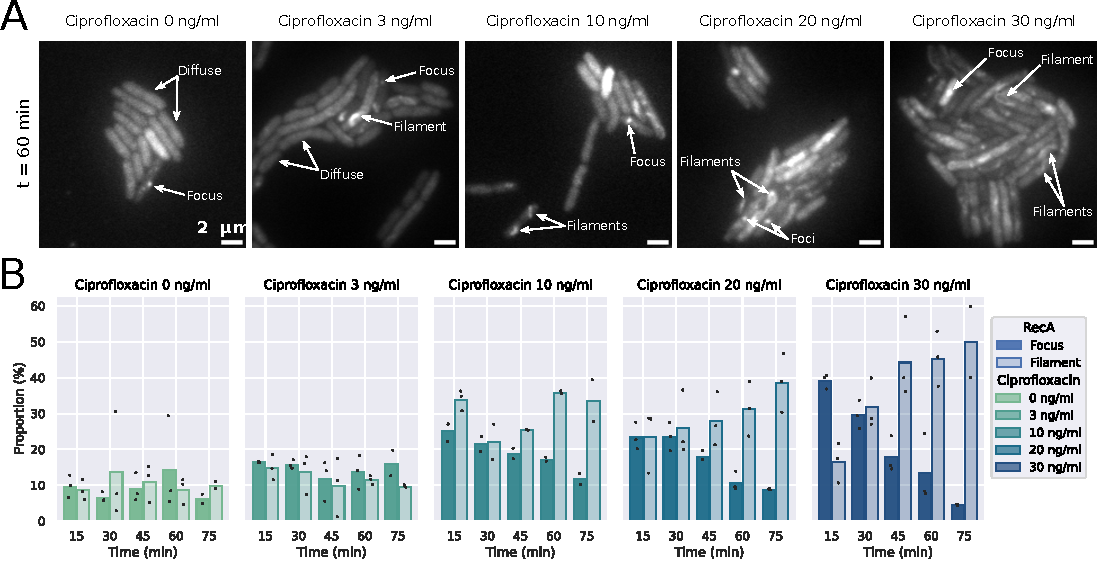
\includegraphics[width=\textwidth]{SI_Figures/RecA_structures.pdf}
    \end{center}
    \caption{RecA structures formed upon exposure to ciprofloxacin. \textbf{(A)} Representative images of cells containing different RecA structures (diffuse fluorescence, foci or filaments) after 60 minutes of exposure to ciprofloxacin. Arrows point to representative examples of each of these structures. \textbf{(B)} Proportion of cells containing RecA foci or filaments. Black dots represent averages for individual datasets, and bars the average between them.\ \ncells{32,031}.}\label{SIFig:reca_structures}
\end{suppfigure*}

% Effect of DSBs on the cell: nucleoid compaction
\begin{suppfigure*}[htbp]
    \begin{center}
    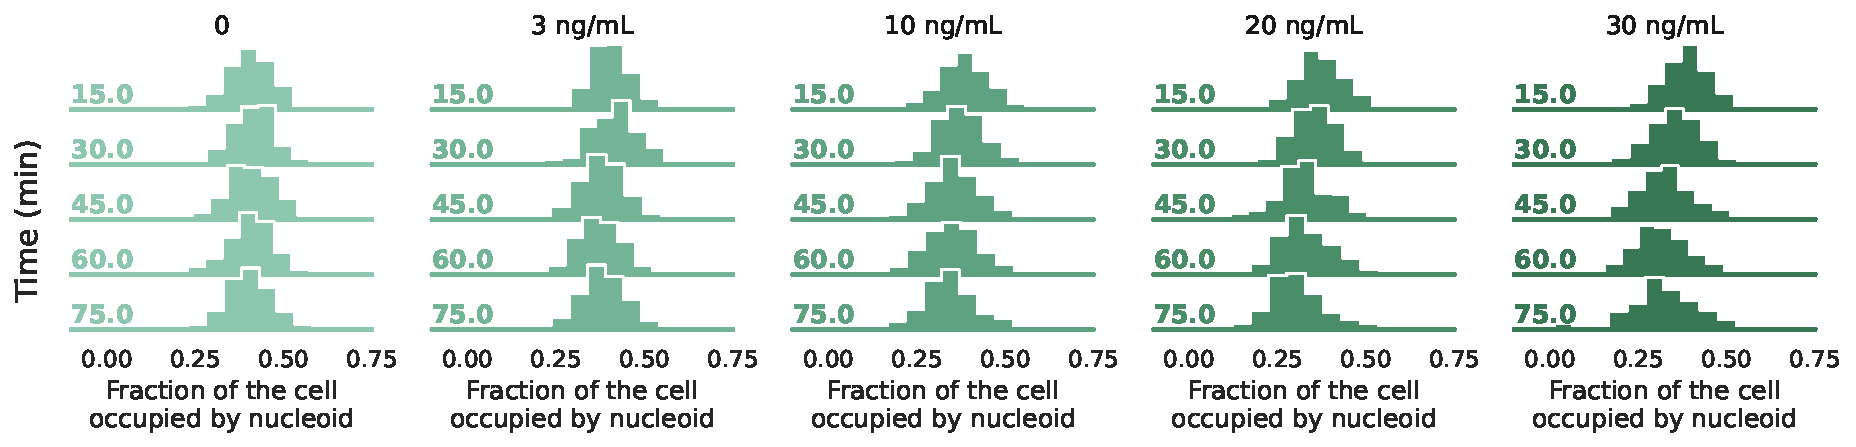
\includegraphics[width=\textwidth]{SI_Figures/Nucleoid_compaction.pdf}
    \end{center}
    \caption{Average fraction of the bacterial cell occupied by the nucleoid (stained using the Sytox Green dye) at different ciprofloxacin concentrations (0 to 30 ng/ml) and duration of exposure (15 to 75 min). Dots represent averages for individual datasets, and dashes the average between them.\ \ncells{24,014}.\ \nnucl{31,441}.}\label{SIFig:nucleoid_compaction}
\end{suppfigure*}

% Effect of DSBs on the cell: nucleoid position
\begin{suppfigure*}[htbp]
    \begin{center}
    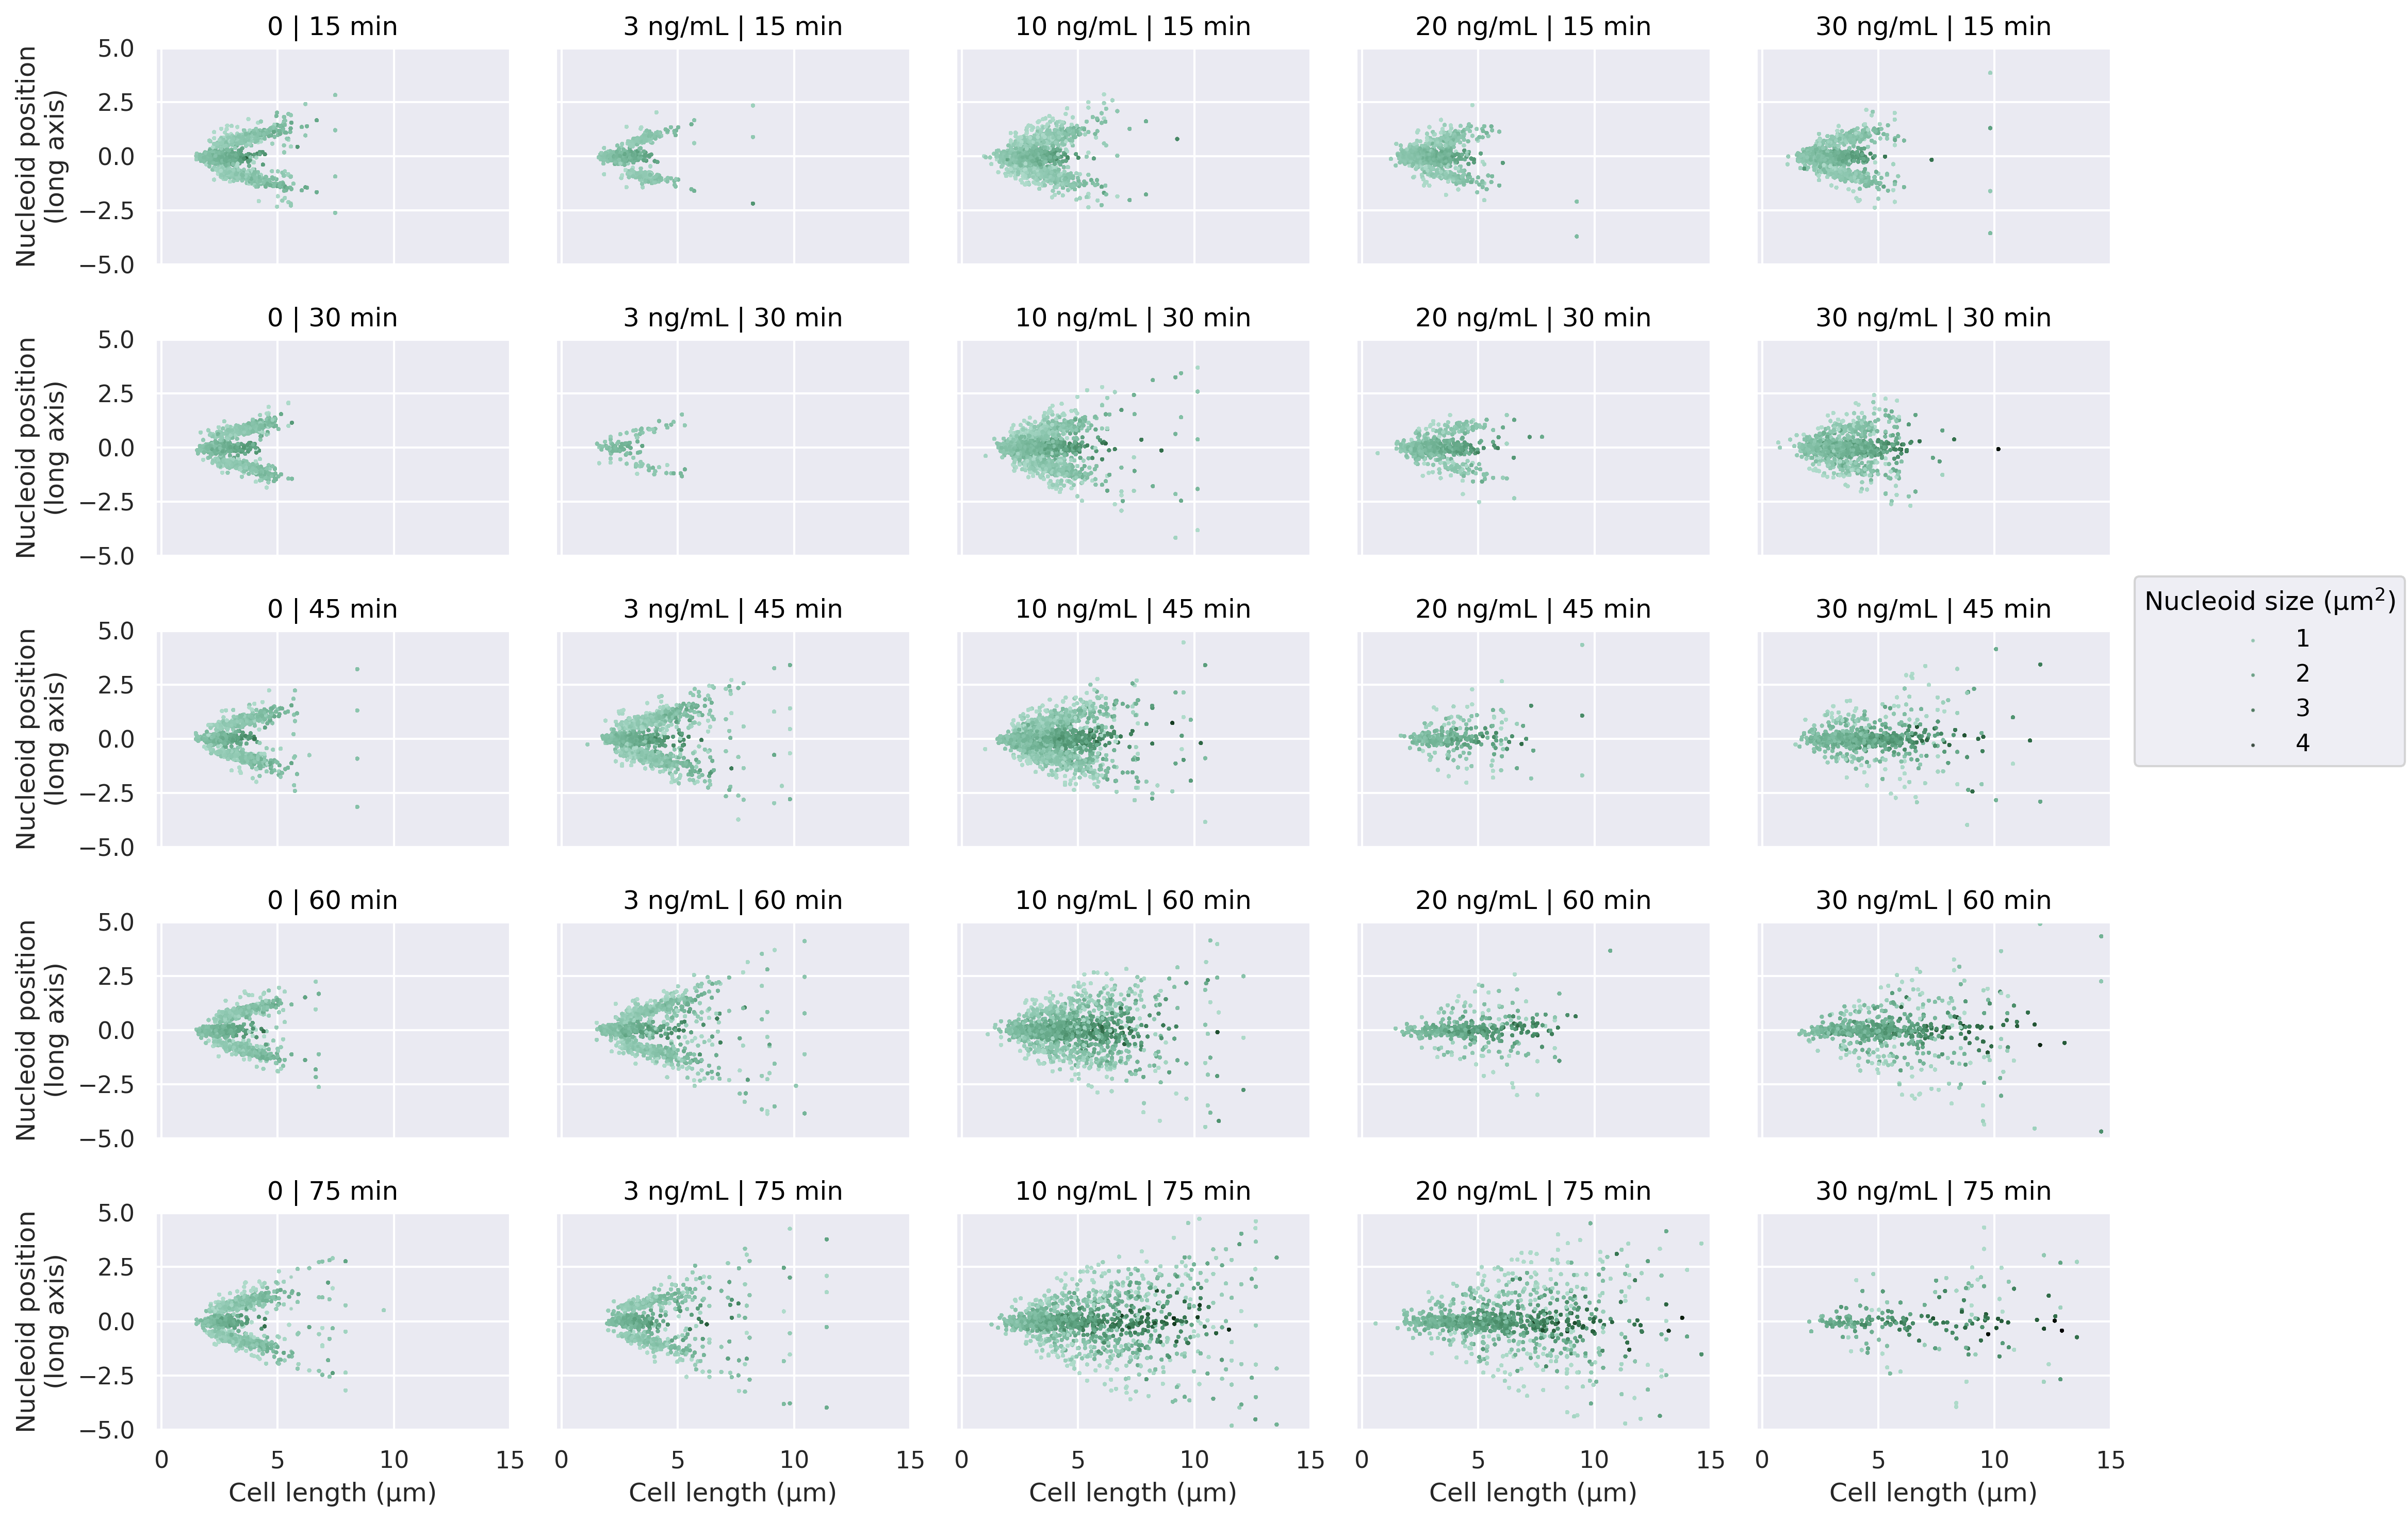
\includegraphics[width=\textwidth]{SI_Figures/Nucleoid_position.png}
    \end{center}
    \caption{Position of the nucleoid along the cell's long axis against cell length for different ciprofloxacin concentrations (columns) and durations of ciprofloxacin exposure (rows). Point colour indicates the total surface covered by the nucleoid in the cell, in \umsq. \ncells{24,014}.\ \nnucl{31,441}.}\label{SIFig:nucleoid_position}
\end{suppfigure*}

% Effect of DSBs on the cell: nucleoid and RecB position overlay separated by timepoints
\begin{suppfigure*}[htbp]
    \begin{center}
    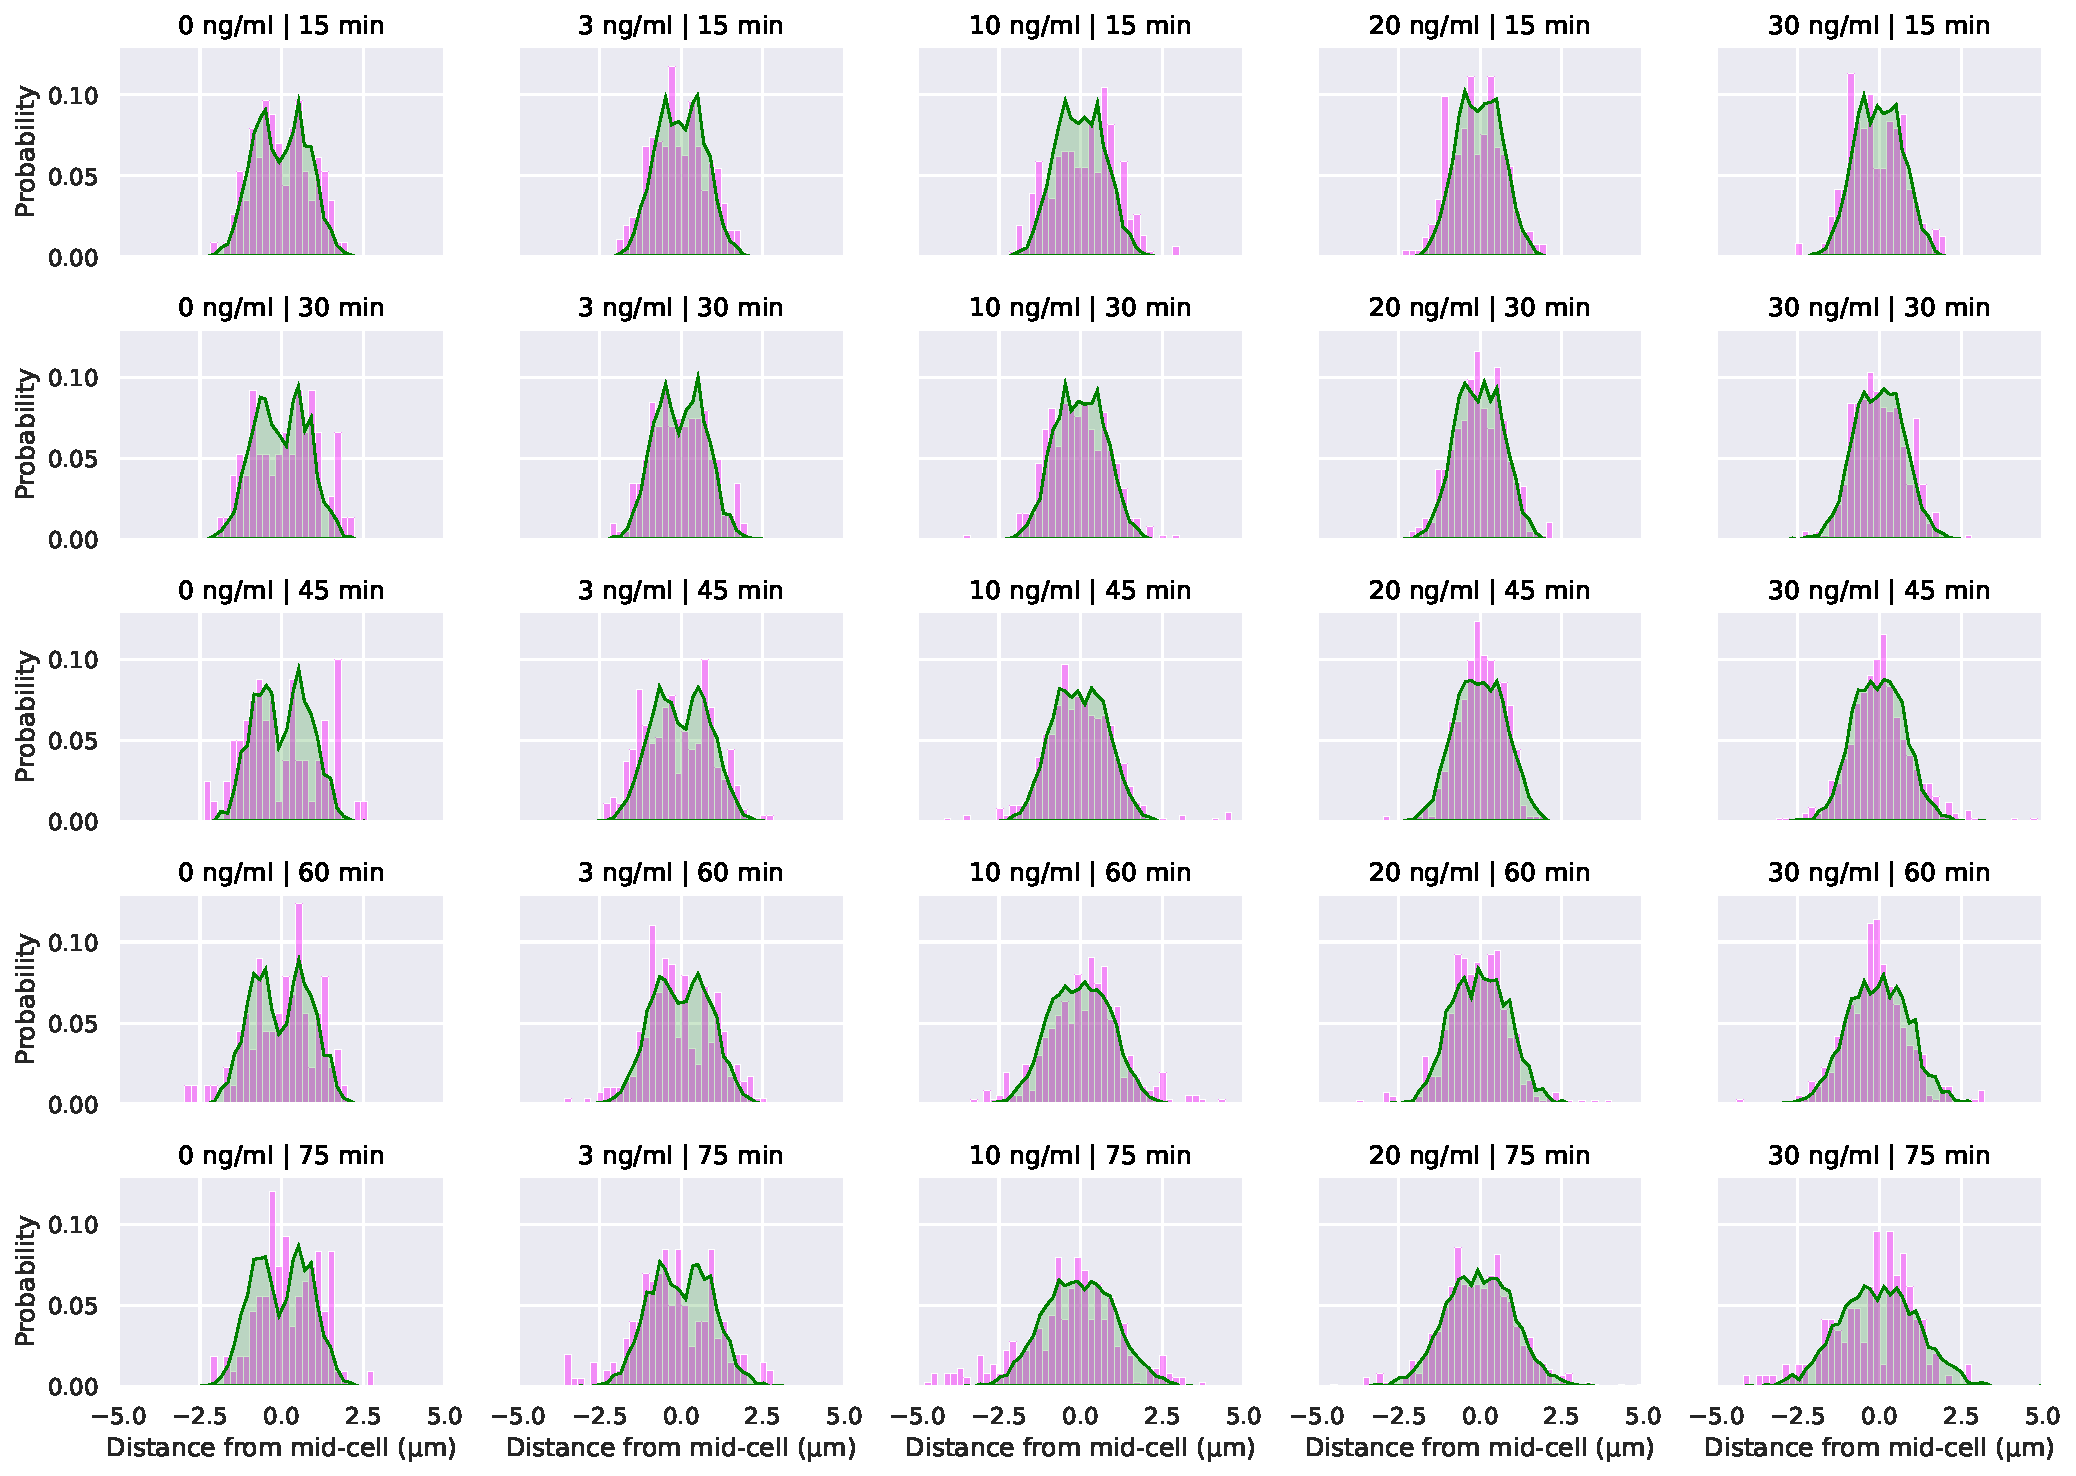
\includegraphics[width=\textwidth]{SI_Figures/RecB_Nucleoid_position_timepoints.pdf}
    \end{center}
    \caption{Overlay of nucleoid density (green area) and position of DSB-bound RecB molecules (magenta bars) along the cell's long axis, for different ciprofloxacin concentrations (columns) and durations of exposure (rows).\ \ncells{15,029}.\ \nspots{58,331}.\ \nnucl{20,831}.}\label{SIFig:recb_nucleoid_timepoints}
\end{suppfigure*}

% Mutants: nucleoid compaction
\begin{suppfigure*}[htbp]
    \begin{center}
    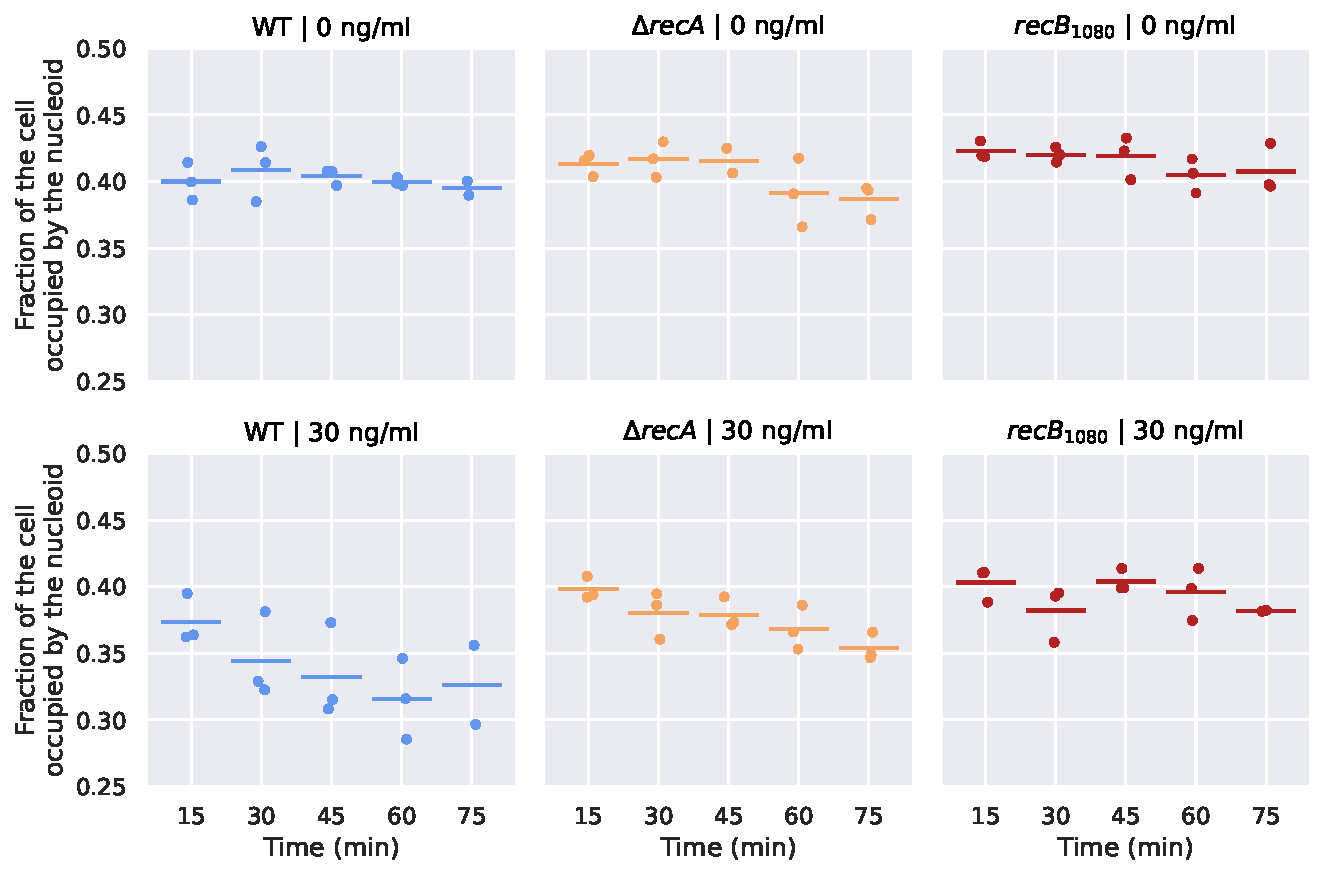
\includegraphics[width=.8\textwidth]{SI_Figures/Mutants_nucleoid_compaction.pdf}
    \end{center}
    \caption{Average fraction of the bacterial cell occupied by the nucleoid (stained using the Sytox Green dye) at different ciprofloxacin concentrations (0 to 30 ng/mL) and duration of exposure (15 to 75 min), for wild-type cells (reproduced from Supp. Figure~\ref{SIFig:nucleoid_compaction} for comparison) and the \dreca\ and \geneteneighty\ mutants. Dots represent averages for individual datasets, and dashes the average between them.\ \ncells{15,029}.\ \nnucl{20,831}.}\label{SIFig:mutants_nucleoid_compaction}
\end{suppfigure*}


\end{document}
